%_________________________________________Heading_______________________________________________%

\documentclass[11pt]{article}
% #1-Asignatura
% #2-Curso
% #3-Nombre
% #4-Link
% #5-Foto

\newcommand{\portada}[5]{
    \begin{titlepage}
        \begin{center}
            \vspace*{0.5cm}
            
            % Titulo con #1 lo mas grande posible
            {\Huge \textbf{#1}}

            
            \vspace{0.5cm}
            \LARGE
            Curso #2 
            
            \vspace{1cm}
            
            \Huge{\textbf{Grupo Viterbi}}

            \vspace{1cm}
            
\includegraphics[width=0.6\textwidth]{assets/Img/UGR-Logo.png}
            
            \vspace{0.5cm}

            \huge
            PRÁCTICA 5- PROGRAMACIÓN DINÁMICA
            
            \Large
            \vspace{1cm}
            \textbf{Integrantes:}  \\ 
             % Array con los nombres de los integrantes y el correo
             \begin{center}
                \begin{tabular}{c c }
                    \textbf{Miguel Ángel De la Vega Rodríguez} & miguevrod@correo.ugr.es \\
                    \textbf{Alberto De la Vera Sánchez} & joaquinrojo724@correo.ugr.es \\
                    \textbf{Joaquín Avilés De la Fuente} & adelaveras01@correo.ugr.es \\
                    \textbf{Manuel Gomez Rubio} & e.manuelgmez@go.ugr.es \\
                    \textbf{Pablo Linari Perez} & e.pablolinari@go.ugr.es
                \end{tabular}
             \end{center}
            \vspace{0.8cm}
            
            
            \large
             \vspace{1cm}
            Facultad de Ciencias UGR\\
            Escuela Técnica Ingeniería Informática UGR\\
            Granada\\
            #2 
            
        \end{center}
    \end{titlepage}
}



\usepackage{assets/formulas}
\usepackage{float}
\usepackage{colortbl}

\usepackage{xcolor}
\hbadness=10000 % Suppress Underfull \hbox warnings

%_________________________________________Indice:_______________________________________________%
\begin{document}                                                
\portada{Algorítmica}{2023-2024}{Miguel Ángel De la Vega Rodríguez}{https://github.com/Miguevrgo/}{github.png}

\tableofcontents % Índice

\newpage %Salto de pagina tras el Indice

%________________________________________Documento:_____________________________________________%
\section{Participación}
\begin{itemize}
    \item \textbf{Miguel Ángel De la Vega Rodríguez:} 20\%
    \begin{itemize}
        \item Plantilla y estructura del documento \LaTeX
        \item Cómputo de la eficiencia de los algoritmos de ordenación
        \item Diseño de main para los ejecutables y scripts
    \end{itemize}
    \item \textbf{Joaquín Avilés De la Fuente:} 20\%
    \begin{itemize}
        \item Diseño del estudio
        \item Computo algoritmo individual
        \item Eficiencia Teórica
    \end{itemize}
    \item \textbf{Alberto De la Vera Sánchez: } 20\%
    \begin{itemize}
        \item Estudio híbrido 
        \item Conclusión
        \item Computo algoritmo individual
    \end{itemize}
    \item \textbf{Manuel Gomez Rubio} 20\%
    \begin{itemize}
        \item Diseño de main para ejecutables (especialmente string)
        \item Computo algoritmo individual
        \item Eficiencia teórica
    \end{itemize}
    \item \textbf{Pablo Linari Pérez:} 20\%
    \begin{itemize}
        \item Estudio y comparación de las gráficas
        \item Diseño del estudio y tablas
    \end{itemize}
\end{itemize}

\section{Equipo de trabajo}

\begin{itemize}
    \item \textbf{Miguel Ángel De la Vega Rodríguez:} (Ordenador donde se ha realizado el computo)
        \begin{itemize}
            \item AMD Ryzen 7 2700X 8-Core
            \item 16 GB RAM DDR4 3200 MHz
            \item NVIDIA GeForce GTX 1660 Ti 
            \item 1 TB SSD NvMe 
        \end{itemize}
\end{itemize}

\section{Objetivos}
    En esta práctica, se han implementado los siguientes algoritmos de ordenación: \textbf{quicksort, mergesort, inserción, burbuja,}
    y \textbf{selección}. Además, se han implementado los algoritmos de \textbf{Floyd}, que calcula el costo del camino mínimo entre cada par de nodos 
    de un grafo dirigido, de \textbf{Fibonacci}, que calcula los números de la sucesión de Fibonacci , y de \textbf{Hanoi}, que resuelve el famoso 
    problema de las torres de Hanoi. Se ha aplicado la siguiente metodología:
    \begin{itemize}
        \item En primer lugar, aunque tenemos la eficiencia teórica de estos algoritmos, se realizarán los calculos necesarios para demostrar
        como se obtiene dicha eficiencia utilizando los distintos métodos estudiados en teoría. \\
        
        \item En segundo lugar, se pasará al estudio empírico de los algoritmos de ordenación de vectores para distintos tipos de datos, es decir, 
        para datos tipo \textbf{int}, \textbf{float}, \textbf{double} y \textbf{string}. Posteriormente, se creará las gráficas para
        cada algoritmo en las que visualizaremos el tiempo de ejecución en función del tamaño del vector y del tipo de dato. Finalmente 
        para esta parte, se hara un calculo de \textbf{eficiencia híbrida} que se basa en ajustar la gráfica obtenida a la función de su eficiencia
        teórica por mínimos cuadrados, obteniendo por tanto los literales de dicha función que ajustan la gráfica.\\
        
        \item En tercer lugar, se hará el estudio de los otros tres algoritmos de forma similar, es decir, se estudiará la eficiencia
        de estos de modo empírica, cuyo estudio se mostrará en las gráficas, y se calculará la eficiencia híbrida de estos, a partir
        de la eficiencia teórica.\\     
    \end{itemize}
\section{Diseño del estudio}

    Los estudios empíricos han sido realizados en el ordenador con las características mencionadas anteriormente.
    Además, hemos realizado el estudio empírico de forma aislada para el algoritmo de ordenación de vectores
    quicksort en los distintos ordenadores de los participantes del grupo para ver como afectan las características
    hardware de cada ordenador en el tiempo de ejecución, cuyas gráficas se mostrarán en la sección de Algoritmos. \\
    En ambos casos se ha hecho uso del sistema operativo Linux, concretamente de Debian, y se ha utilizado el
    compilador gcc para la compilación de los programas  con el flag -Og para la optimización.
    \subsection{Algoritmos de ordenación de vectores}
    Para los algoritmos de ordenación se han usado entradas de datos de tipo int, float, double y string mientras que para los algoritmos de Hanoi, Floyd  y Fibonnaci solo se han usado entradas de tipo int 
    ya que no tendría sentido usar entradas de otro tipo. 
    \begin{itemize}
        \item En los algoritmos con eficiencia  \(O(n^2)\) como los de Burbuja, Selección e Inserción los saltos usados entre los tipos de datos int, float y double generados aleatoriamente son de 5000 en 5000 empezando con una muestra de 5000 datos y llegando a
        un máximo de 125000 datos.
        \item En los lagoritmos con eficiencia \(O (n\log(n))\) como el mergesort o el quicksort los saltos usados entre los tipos de datos int, float y double generados aleatoriamente son de 50000 en 50000 empezando con una muestra de 50000 datos y llegando a
        un máximo de 1250000 datos.
    \end{itemize}

    \subsection{Otros algoritmos}
    En los algoritmos restantes se han usado datos de tipo int generados aleatoriamente y proporcionados en la siguiente medida:
    \begin{itemize}
        \item Para el algoritmo de \textit{Floyd}  que es de orden \(O(n^3)\) se han usado enteros aleatorios desde 50 hasta 1250 con saltos de 50 en 50.
        \item Para el algoritmo de \textit{Fibonnaci}  que es de orden \(O((\frac{1+\sqrt{5}}{2})^n\)) se han usado enteros aleatorios desde 50 hasta 1250 con saltos de 50 en 50.
        \item Para el algoritmo de \textit{Hanoi} que es de orden \(O(2^n)\) se han usado enteros aleatorios desde 3 hasta 33 con saltos de 50 en 50. 
    \end{itemize}

    Por último para el tipo de dato string se han extraido las muestras del archivo \textit{quijote.txt} para simular una generación aleatoria de palabras, 
    esta entrada de datos no ha sido totalmente aleatoria ya que al usar un lenguaje determinado para el texto, en este caso el español, se repiten con mas frecuencia algunas palabras por tanto esto se verá 
    reflejado en el comportamiento de los  algoritmos. En este caso el Quijote tiene un total de 202308 palabras por lo que se comenzará con una muestra de 12308 palabras con saltos de 
    10000 en 10000 hasta llegar a 202308 palabras.
    \subsection{Scripts usados para la ejecución}
    \begin{itemize}
        \item \textbf{[AutoCompile.sh]} Este script se encarga de compilar todos los ficheros en una misma carpeta con las mismas
        opciones de compilación, para garantizar la máxima igualdad posible entre cada algoritmo y organizar la estructura de 
        ficheros.
        \item \textbf{[AutoFinal.sh]} Este script es el encargado de ejecutar todos los algoritmos varias veces con las opciones respectivas para cada uno,
        el resultado se pasa por un programa AutoMedia.py que se encarga de realizar la media de las ejecuciones de los algoritmos,
        este resultado es guardado en una carpeta llamada Resultados de la que posteriormente el mismo script genera las graficas
        de cada algoritmo.
        \item \textbf{[AutoIndividual.sh]} Este script es como el descrito previamente pero unicamente ejecuta un script, esto ha sido útil para hacer
        pruebas sin la necesidad de esperar la gran cantidad de tiempo que requiere la ejecución de todos los algoritmos.
        \item \textbf{[AutoHibrido.sh]} Este script se encarga de generar las gráficas de los ajustes híbridos, así como de guardar en un fichero .log los
        resultados numéricos de ajustar las gráficas. De dicho fichero obtenemos las constantes ocultas como la varianza de residuos
    \end{itemize}
    
\section{Algoritmos}
    Esta sección esta dedicada a mostrar los resultados obtenidos en el estudio de los algoritmos,
    la estructura seguida para mostrar los resultados consiste en mostrar, para cada algoritmo, los tiempos 
    de ejecución, junto con las gráficas obtenidas y los ajustes correspondientes. Previo a ello, se analizará
    en cada caso teoricamente la eficiencia prevista para cada algoritmo.

    \subsection{Estudio teórico}
        En esta sección se calculará la eficiencia teórica de cada algoritmo, es decir, la eficiencia que se espera al hacer el
        estudio empírico de cada algoritmo. Para ello, se utilizarán los métodos estudiados en teoría.
        \subsection*{Algoritmo de ordenación Burbuja}
        Utilizaremos el siguiente fragmento de código para estudiar su eficiencia, pues es el utilizado en la práctica
        \begin{lstlisting}
            void burbuja(int T[], int inicial, int final)
            {
            int i, j;
            int aux;
            for (i = inicial; i < final - 1; i++)
                for (j = final - 1; j > i; j--)
                if (T[j] < T[j - 1])
                {
                    aux = T[j];
                    T[j] = T[j - 1];
                    T[j - 1] = aux;
                }
            }
        \end{lstlisting}
        El trozo de código dentro del bucle interno, es decir, de la línea 7 a la 12 tiene eficiencia $O(1)$ y por tanto
        tiene un tiempo de ejecución constante que anotaremos como $a$. Además, este trozo de código se ejecuta
        en concreto $(final-1)-(i+1) +1$ veces, es decir, $final-i+1$ veces. Es claro que la ejecución de la línea 3 y 4 
        y las comparaciones, inicializaciones y actualizaciones de los bucles tienen eficiencia $O(1)$. Sabiendo esto y que 
        el número de veces que se ejecute el bucle interno depende del externo tenemos entonces la siguiente fórmula 
        \begin{equation*}
            \sum_{i=inicial}^{final-2} \sum_{j=i+1}^{final-1}a 
        \end{equation*}
        Tomaremos $final =  n$ e $inicial = 1$ para simplificar el cálculo y veamos que obtenemos ahora
        \begin{equation*}\begin{split}
            \sum_{i=1}^{n-2} \sum_{j=i+1}^{n-1}a&= a \cdot \sum_{i=1}^{n-2} \sum_{j=1}^{n-i-1}1
             = a \cdot \sum_{i=1}^{n-2} (n-i-1) a \cdot ( n\sum_{i=1}^{n-2} 1 - \sum_{i=1}^{n-2} i - \sum_{i=1}^{n-2} 1)= \\
            &= a \cdot ( n(n-2) - \frac{(n-2)(n-1)}{2} - (n-2))= a \cdot ( n^2-2n - \frac{n^2-3n+2}{2} - n+2)=\\
            &= a \cdot \left(\frac{n^2}{2}-\frac{3}{2}n+1\right)= \frac{n^2}{2}a-\frac{3}{2}na+a
        \end{split}\end{equation*}
        Es claro que $\frac{n^2}{2}a-\frac{3}{2}na+a \in O(n^2)$ y por tanto la eficiencia teórica del algoritmo de burbuja es $O(n^2)$.

        \subsection*{Algoritmo de ordenación Inserción}
        Utilizaremos el siguiente fragmento de código para estudiar su eficiencia, pues es el utilizado en la práctica
        \begin{lstlisting}
            void insercion(int T[], int inicial, int final)
            {
              int i, j;
              int aux;
              for (i = inicial + 1; i < final; i++) {
                j = i;
                while ((T[j] < T[j-1]) && (j > 0)) {
                  aux = T[j];
                  T[j] = T[j-1];
                  T[j-1] = aux;
                  j--;
                };
              };
            }
            
        \end{lstlisting}
        El trozo de código dentro del bucle interno, es decir, de la línea 8 a la 10 tiene eficiencia $O(1)$ y por tanto
        tiene un tiempo de ejecución constante que anotaremos como $a$. Dicho trozo de código se ejecutará en el peor de los casos
        $i-(0-1)+1=i$ veces, mientras que el bucle while se ejecutará $(final-1)-(inicial+1)+1=final-inicial-1$ veces.
        Sabiendo que la ejecución de la línea 3 y 4 y las comparaciones, inicializaciones y actualizaciones de los bucles tienen eficiencia $O(1)$, 
        tenemos la siguiente fórmula
        \begin{equation*}
            \sum_{i=inicial+1}^{final-1} \sum_{j=1}^{i}a
        \end{equation*}
        Tomaremos $final =  n$ e $inicial = 1$ para simplificar el cálculo y veamos que obtenemos ahora
        \begin{equation*}
            \sum_{i=2}^{n-1} \sum_{j=1}^{i}a= a \cdot \sum_{i=1}^{n-2} \sum_{j=1}^{i}1= a \cdot \sum_{i=1}^{n-2} i
            = a \cdot \frac{(n-2)(n-1)}{2}=\frac{n^2}{2}a-\frac{3n}{2}a+a 
        \end{equation*}
        Es claro que $\frac{n^2}{2}a-\frac{3}{2}na+a \in O(n^2)$ y por tanto la eficiencia teórica del algoritmo de inserción es $O(n^2)$.
        
        \subsection*{Algoritmo de ordenación Selección}
        Utilizaremos el siguiente fragmento de código para estudiar su eficiencia, pues es el utilizado en la práctica
        \begin{lstlisting}
            void seleccion(int T[], int inicial, int final)
            {
              int i, j, indice_menor;
              int menor, aux;
              for (i = inicial; i < final - 1; i++) {
                indice_menor = i;
                menor = T[i];
                for (j = i; j < final; j++)
                  if (T[j] < menor) {
                    indice_menor = j;
                    menor = T[j];
                  }
                aux = T[i];
                T[i] = T[indice_menor];
                T[indice_menor] = aux;
              };
            }
        \end{lstlisting}
        El trozo de código dentro del bucle interno, es decir, de la línea 9 a la 14 tiene eficiencia $O(1)$ y por tanto
        tiene un tiempo de ejecución constante que anotaremos como $a$. Este trozo de código se ejecutará en el peor de los casos
        $(final-1)-i+1=final-i$ veces, mientras que el bucle for interno se ejecutará $(final-1-1)-inicial+1=final -inicial-1$ veces.
        Sabiendo que la ejecución de las líneas 3, 4, 6, 7 y las comparaciones, inicializaciones y actualizaciones de los 
        bucles tienen eficiencia $O(1)$, tenemos la siguien fórmula
        \begin{equation*}
            \sum_{i=inicial}^{final-2} \sum_{j=i}^{final-1}a 
        \end{equation*}
        Tomaremos $final =  n$ e $inicial = 1$ para simplificar el cálculo y veamos que obtenemos ahora
        \begin{equation*}\begin{split}
            \sum_{i=1}^{n-2} \sum_{j=i}^{n-1}a&= a \cdot \sum_{i=1}^{n-2} \sum_{j=1}^{n-1-(i-1)}1
             = a \cdot \sum_{i=1}^{n-2} \sum_{j=1}^{n-i}1=a \cdot \sum_{i=1}^{n-2} n-i= a \cdot (n\sum_{i=1}^{n-2}1 - \sum_{i=1}^{n-2}i) \\
            & = a \cdot\left(n(n-2)-\frac{(n-2)(n-1)}{2}\right)= a \cdot \left(n^2-2n-\frac{n^2-3n+2}{2}\right)= a \cdot \left(\frac{n^2}{2}-\frac{n}{2}+1\right) \\
            & = \frac{n^2}{2}a-\frac{n}{2}a+a
        \end{split}\end{equation*}
        Es claro que $\frac{n^2}{2}a-\frac{n}{2}a+a \in O(n^2)$ y por tanto la eficiencia teórica del algoritmo de inserción es $O(n^2)$.

        \subsection*{Algoritmo de ordenación Mergesort}
        Utilizaremos el siguiente fragmento de código para estudiar su eficiencia, pues es el utilizado en la práctica
        \begin{lstlisting}
  
        void fusion(int T[], int inicial, int final, int U[], int V[])
        {
            int j = 0;
            int k = 0;
            for (int i = inicial; i < final; i++){
                if (U[j] < V[k]) {
                    T[i] = U[j];
                    j++;
                } else{
                    T[i] = V[k];
                    k++;
                };
            };
        }

        void mergesort(int T[], int inicial, int final)
        {
            if (final - inicial < UMBRAL_MS){
                insercion(T, inicial, final);
            } else {
                int k = (final - inicial)/2;

                int * U = new int [k - inicial + 1];
                assert(U);
                int l, l2;
                for (l = 0, l2 = inicial; l < k - inicial; l++, l2++)
                    U[l] = T[l2];
                U[l] = INT_MAX;

                P * V = new P [final - k + 1];
                assert(V);
                for (l = 0, l2 = k; l < final - k; l++, l2++)
                    V[l] = T[l2];
                V[l] = INT_MAX;

                mergesort_lims(U, 0, k - inicial);
                mergesort_lims(V, 0, final - k);
                fusion(T, inicial, final, U, V);
                delete [] U;
                delete [] V;
            };
        }
        \end{lstlisting}
        Destacar que tomaremos \textit{final =n} e \textit{inicial=0}. Es claro que en el caso de \textit{n=final-inicial}$<\nobreak UMBRAL\_MS$ 
        la eficiencia del algoritmo en el peor caso es $O(UMBRAL\_MS^2)$, es decir, constante, por tanto, nos centraremos en el caso en el que $n\geq UMBRAL\_MS$.
        En este caso, el algoritmo se divide en dos partes, la primera parte es la creación de los vectores $U$ y $V$ y la segunda parte es la
        llamada recursiva a la función mergesort y el resto de código. \\
        La primera parte la podemos dividir en dos: la creación del vector $U$ tomando entonces de la línea 22 a la línea
        29, donde podemos ver que el bucle for de la línea 27 se ejecuta $\frac{n}{2}$ veces; y la creación del vector 
        $V$ tomando entonces de la línea 31 a la línea 35, donde tenemos el mismo resultado. Tenemos entonces que ambas partes 
        tienen eficiecia $O(\frac{n}{2})$, es decir, $O(n)$ y aplicando la regla del máximo obtendríamos hasta la línea 35 un
<<<<<<< HEAD
        orden de $O(n)$. \\
        En la segunda parte, observamos que la llamada recursiva a la función mergesort se hace dos veces con vectores de tamaño $\frac{n}{2}$.
        Además, viendo la función \textbf{fusion} vemos que el bucle for de la línea 6 se ejecuta $n$ veces, es decir, dicha función
        tiene eficiencia $O(n)$. \\
        Teniendo en cuenta el razonamiento hecho y aplicando la regla de la suma, obtenemos la siguiente ecuación
        \begin{equation*}
            T(n)=2T(\frac{n}{2})+n
        \end{equation*}
        Pasemos ahora a resolver dicha ecuación de recurrencia. Aplicando el siguiente cambio de variable $n=2^m$ obtenemos
        \begin{equation*}
            T(2^m)=2T(2^{m-1})+2^m \Longrightarrow T(2^m)-2T(2^{m-1})=2^m
        \end{equation*}
        Resolvamos la parte homógenea de la ecuación, es decir, la ecuación $T(2^m)-2T(2^{m-1})=0$. Obtenemos el polinomio
        característico de la parte homógenea que es $p_H(x)=x-2$ cuya raíz es $x=2$. \\
        Obtengamos ahora la parte no homógenea
        \begin{equation*}
            2^m=b_1^m q_1(m) \Longrightarrow b_1=2 \wedge q_1(m)=1 \text{ con grado } d_1=0
        \end{equation*}
        Tenemos entonces el siguiente polinómio característico
        \begin{equation*}
            p(x)=(x-2)(x-b_1)^{d_1+1}=(x-2)^2
        \end{equation*}
        Por tanto la solución general es
        \begin{equation*}
            t_m=c_{10}2^mm^0+c_{11}2^mm^1  \overset{*}{\Longrightarrow}  t_n=c_{10}n+c_{11}n\log_2(n) \Longrightarrow T(n)=c_{10}n+c_{11}n\log_2(n)
        \end{equation*}
        donde en ($*$) hemos deshecho el cambio de variable \\
        Aplicando la regla del máximo tenemos $T(n) \in O(n\log(n))$

        \subsection*{Algoritmo de ordenación quicksort}
        Para el estudio de eficiencia de este algoritmo hemos usado el siguiente código:
        \begin{lstlisting}
        void quicksort(int T[], int inicial, int final){
            int k;
            if (final - inicial < UMBRAL_QS) {
                insercion(T, inicial, final);
            } else {
                dividir_qs(T, inicial, final, k);   <--- O(n)

                //peor caso    
                0(n-1) ---> quicksort(T, inicial, k);  <--- O(n/2)
                0(1) ---> quicksort(T, k + 1, final);  <--- O(n/2)
            }
        }

        void dividir_qs(int T[], int inicial, int final, int & pp){
            int pivote, aux;
            int k, l;

            pivote = T[inicial];
            k = inicial;
            l = final;
            do {
                k++;
            } while ((T[k] <= pivote) && (k < final-1));   <--- O(n)
            do {
                l--;
            } while (T[l] > pivote);
            while (k < l) {            <--- O(n)
                aux = T[k];
                T[k] = T[l];
                T[l] = aux;
                do k++; while (T[k] <= pivote);
                do l--; while (T[l] > pivote);
            };
            aux = T[inicial];
            T[inicial] = T[l];
            T[l] = aux;
            pp = l;
        };
        \end{lstlisting}
        Para el estudio de la eficiencia se ha ido estudiando cada método por separado. El método llamado inserción 
        no se tiene en cuenta para la eficiencia ya que solo se usa cuando el problema es de un tamaño menor a UMBRAL\_QS.\\
        A simple vista es fácil comprobar que el propósito del algoritmo es dividir la ordenación del vector de tamaño
        original en otros dos de un tamaño más reducido, en el mejor de los casos este será a la mitad si el pivote es 
        justo la mediana. La parte de la llamada recursiva, es $O(\frac{n}{2})$, y la llamada a dividir\_qs es $O(n)$, por tanto obtenemos
        la siguiente expresión:
        \begin{equation*}
            T(n) = 2 T\left(\frac{n}{2}\right) + n
        \end{equation*}
        usando el cambio de variable $n=2^k$ obtenemos:
        \begin{equation*}
            t_k - 2t_{k-1} = 2^k 
        \end{equation*}
        cuyo polinomio característico es: $$p(x)=(x-2)^2 \Rightarrow t_k=c_1 2^k + c_2 2^k k$$
        Finalmente, desacemos el cambio obteniendo: 
        \begin{equation*}
            t_n = c_1 n + c_2 n log_2 n \in O(nlog_2 n)
        \end{equation*}
        Donde vemos que el algorimo es $O(nlog n)$.\\
        En el peor caso, lo que ocurre es que el algoritmo no puede establecer un buen pivote, lo que hace que se obtenga la siguiente
        ecuación:
        \begin{equation*}
            T(n)=T(n-1)+n+1= T(n-2)+2n+2=...=T(n-k)+kn+k
        \end{equation*}
        tomando $k=n-1$ para llegar al caso base tenemos que:
        \begin{equation*}
            T(n)=T(n-n+1)+(n-1)n+n-1=T(1)+(n-1)n+n-1 \in O(n^2)
        \end{equation*}
        Donde se ve que en el peor de los casos el algoritmo es $O(n^2)$ que es lo que ocurre con los string por tener un mayor coste de 
        operación, o con los vectores de números ya ordenados o casi ordenados.

        \subsection*{Algoritmo de Floyd}
        Para analizar la eficiencia de este algoritmo se ha usado este fragmento del código:
        \begin{lstlisting}
        void Floyd(int **M, int dim){
        for (int k = 0; k < dim; k++)
            for (int i = 0; i < dim;i++)
                for (int j = 0; j < dim;j++)
                {
                int sum = M[i][k] + M[k][j];    	
                  M[i][j] = (M[i][j] > sum) ? sum : M[i][j];
            }
        }	     	
        \end{lstlisting}
        Para el estudio de la eficiencia de este algoritmo es bastante simple ya que a simple vista ya se puede comprobar que es $O(n^3)$ porque hay 
        tres bucles for anidados y cada uno es $O(n)$ por lo que el algoritmo es $O(n^3)$ como se había mencionado.
        $$T(n) \in O(n^3)$$

        \subsection*{Algoritmo de Fibonacci}
        Para el la estudio de la eficiencia de este algoritmo se ha usado el siguiente código:
        \begin{lstlisting}
        int fibo(int n){
            if (n < 2)
                return 1;
            else
                return fibo(n-1) + fibo(n-2);
        }
            
        \end{lstlisting}

        Estudiando este código se pueden observar dos llamadas recursivas con n-1 y n-2 respectivamente, por lo que si obtenemos la ecuación
        de la eficiencia del algorimo, al ser la condición del if constante, tenemos que:
        \begin{equation*}
            T(n)=T(n-1)+T(n-2)+1
        \end{equation*}
        tomando $T(n)=x^n$ obtenemos:
        \begin{equation*}
            x^n = x^{n-1} + x^{n-2} + 1 \Leftrightarrow x^n - x^{n-1} - x^{n-2} = 1 \Leftrightarrow x^{n-2}(x^2-x-1) = 1 = 1^n n^0
        \end{equation*}
        como $x^{n-2}\neq 0$ tenemos que calcular las raíces del polinomio característico:
        \begin{equation*}
            p(x) = (x-\frac{1+\sqrt{5}}{2})(x-\frac{1-\sqrt{5}}{2})(x-1)
        \end{equation*}
        de donde obtenemos:
        \begin{equation*}
            t(n) = c_1 \left(\frac{1+\sqrt{5}}{2}\right)^n +c_2 \left(\frac{1-\sqrt{5}}{2}\right)^n +c_3 1^n \Rightarrow T(n) \in O\left(\left(\frac{1+\sqrt{5}}{2}\right)^n\right)
        \end{equation*}
        Por tanto se comprueba que el algoritmo es $O((\frac{1+\sqrt{5}}{2})^n)$
    
        \subsection*{Algoritmo de Hanoi}
        Para el la estudio de la eficiencia de este algoritmo se ha usado el siguiente código:
        \begin{lstlisting}
            void hanoi (int M, int i, int j){
                if (M > 0)
                    {
                    hanoi(M-1, i, 6-i-j);
                    hanoi (M-1, 6-i-j, j);
                }
            }
        \end{lstlisting}
        Vemos que se llama recursivamente dos veces a la función hanoi con M-1, y sabiendo que la eficiencia del if es constante tenemos 
        la siguiente ecuación de recurrencia:
        \begin{equation*}
            T(n)=2T(n-1)+1 \wedge T(0)=1
        \end{equation*}
        Destacar que hemos tomado n=M. Resolviendo la ecuación de recurrencia obtenemos:
        \begin{equation*}\begin{split}
            T(n)=2T(n-1)+1
            &=2(2T(n-2)+1)+1=2^2T(n-2)+3=2(2^2T(n-3)+3)+1=2^3T(n-3)+7= \\
            &=...=2^kT(n-k)+2k-1
        \end{split}\end{equation*}
        Habiendo obtenido el caso general, veamos que obtenemos con $k=n$
        \begin{equation*}
            T(n)=2^nT(n-n)+2n-1=2^{n}T(0)+2n-1=2^n+2n-1 \Longrightarrow T(n)\in O(2^n)
        \end{equation*}
        Por tanto se comprueba que el algoritmo es $O(2^n)$
\subsection{Estudio empírico}
A continuación pasamos a estudiar la eficiencia empírica de los algoritmos previamente vistos, el objetivo de este estudio es ver el comportamiento real 
de los algoritmos al ser ejecutados en un ordenador.Se presentaran los datos en dos formatos grafica y tabla para poder contrastar visualmente los algoritmos.

\subsection*{Burbuja}
Como se puede observar, el algoritmo de burbuja es \(O(n^2)\) y su eficiencia con datos numéricos es parecida en los tres
tipos, mientras que con datos de tipo string se observa un mayor costo de tiempo de ejecución.

\begin{figure}[H]
    \begin{minipage}{0.5\textwidth}
        \centering
        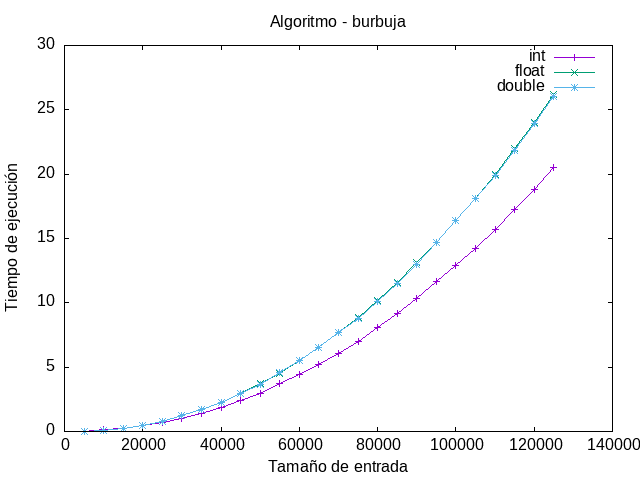
\includegraphics[width=\linewidth]{assets/Img/burbuja.png}
        \caption{Ejecución algoritmo burbuja}
        \label{fig:burbuja}
    \end{minipage}%
    \begin{minipage}{0.5\textwidth}
        \centering
        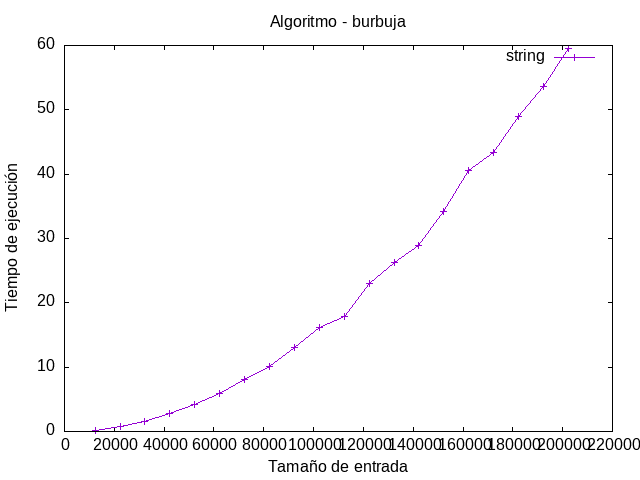
\includegraphics[width=\linewidth]{assets/Img/burbujastring.png}
        \caption{Ejecución algoritmo burbuja con string}
        \label{fig:burbujastring}
    \end{minipage}
\end{figure}
\begin{table}[!ht]
    \centering
    \small
    \begin{tabular}{|l|l|l|l|l|l|l|l|}
    \hline
    \multicolumn{8}{|c|}{\cellcolor{blue!20}\textbf{Burbuja}} \\ \hline
    \multicolumn{2}{|c|}{\cellcolor{gray!20}Tipo Int} & \multicolumn{2}{c|}{\cellcolor{gray!20}Tipo Float} & \multicolumn{2}{c|}{\cellcolor{gray!20}Tipo Double} & \multicolumn{2}{c|}{\cellcolor{gray!20}Tipo String}\\ \hline
        \textbf{Tamaño} & \textbf{Tiempo} & \textbf{Tamaño} & \textbf{Tiempo} & \textbf{Tamaño} & \textbf{Tiempo} & \textbf{Tamaño} & \textbf{Tiempo} \\ \hline
        5000 & 0,0349211 & 5000 & 0,0217027 & 5000 & 0,021847 & 12308 & 0,211221 \\ \hline
        10000 & 0,120458 & 10000 & 0,102747 & 10000 & 0,101877 & 22308 & 0,615473 \\ \hline
        15000 & 0,245185 & 15000 & 0,258293 & 15000 & 0,25446 & 32308 & 1,28107 \\ \hline
        20000 & 0,441264 & 20000 & 0,492039 & 20000 & 0,49134 & 42308 & 2,1949 \\ \hline
        25000 & 0,683406 & 25000 & 0,812521 & 25000 & 0,802523 & 52308 & 3,34899 \\ \hline
        30000 & 1,04181 & 30000 & 1,20884 & 30000 & 1,22906 & 62308 & 4,76194 \\ \hline
        35000 & 1,38162 & 35000 & 1,69518 & 35000 & 1,69937 & 72308 & 6,41449 \\ \hline
        40000 & 1,84603 & 40000 & 2,27424 & 40000 & 2,25218 & 82308 & 8,29372 \\ \hline
        45000 & 2,38588 & 45000 & 2,93436 & 45000 & 2,91507 & 92308 & 10,4296 \\ \hline
        50000 & 2,98525 & 50000 & 3,69289 & 50000 & 3,66562 & 102308 & 12,827 \\ \hline
        55000 & 3,69388 & 55000 & 4,53819 & 55000 & 4,58012 & 112308 & 15,4556 \\ \hline
        60000 & 4,39556 & 60000 & 5,52096 & 60000 & 5,49872 & 122308 & 18,6297 \\ \hline
        65000 & 5,17327 & 65000 & 6,56449 & 65000 & 6,50195 & 132308 & 21,4492 \\ \hline
        70000 & 6,06058 & 70000 & 7,6747 & 70000 & 7,66039 & 142308 & 25,1843 \\ \hline
        75000 & 7,0144 & 75000 & 8,89351 & 75000 & 8,79687 & 152308 & 28,8384 \\ \hline
        80000 & 8,04692 & 80000 & 10,2096 & 80000 & 10,1098 & 162308 & 32,7271 \\ \hline
        85000 & 9,15881 & 85000 & 11,6127 & 85000 & 11,5094 & 172308 & 36,8875 \\ \hline
        90000 & 10,3159 & 90000 & 13,1071 & 90000 & 12,9876 & 182308 & 41,3668 \\ \hline
        95000 & 11,6496 & 95000 & 14,6642 & 95000 & 14,7154 & 192308 & 46,0167 \\ \hline
        100000 & 12,8843 & 100000 & 16,3917 & 100000 & 16,3819 & 202308 & 50,8681 \\ \hline
        105000 & 14,2458 & 105000 & 18,1445 & 105000 & 18,1415 & ~ & ~ \\ \hline
        110000 & 15,7108 & 110000 & 19,9994 & 110000 & 19,9348 & ~ & ~ \\ \hline
        115000 & 17,2545 & 115000 & 21,9713 & 115000 & 21,8762 & ~ & ~ \\ \hline
        120000 & 18,8423 & 120000 & 24,0176 & 120000 & 23,9177 & ~ & ~ \\ \hline
        125000 & 20,5122 & 125000 & 26,1758 & 125000 & 26,0694 & ~ & \\\hline
    \end{tabular}
\end{table}


\subsection*{Seleccion}
El algoritmo de seleccion es \(O(n^2)\) y su eficiencia con datos numéricos es parecida en los tres
tipos pero en este caso los datos de tipo int sacan mas ventaja que los tipo float , mientras que con datos de tipo string se observa un mayor costo de tiempo de ejecución.
\begin{figure}[H]
    \begin{minipage}{0.5\textwidth}
        \centering
        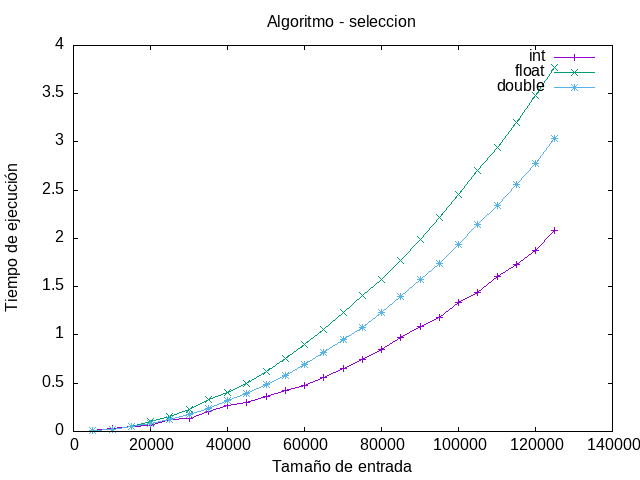
\includegraphics[width=\linewidth]{assets/Img/seleccion.png}
        \caption{Ejecución algoritmo seleccion}
        \label{fig:seleccion}
    \end{minipage}%
    \begin{minipage}{0.5\textwidth}
        \centering
        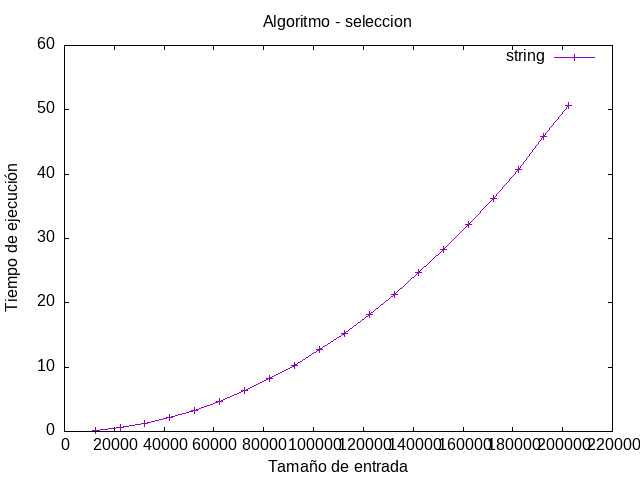
\includegraphics[width=\linewidth]{assets/Img/seleccionstring.png}
        \caption{Ejecución algoritmo seleccion con string}
        \label{fig:seleccionstring}
    \end{minipage}
\end{figure}

\begin{table}[!ht]
    \centering
    \small
    \begin{tabular}{|l|l|l|l|l|l|l|l|}
    \hline
    \multicolumn{8}{|c|}{\cellcolor{blue!20}\textbf{Selección}} \\ \hline
    \multicolumn{2}{|c|}{\cellcolor{gray!20}Tipo Int} & \multicolumn{2}{c|}{\cellcolor{gray!20}Tipo Float} & \multicolumn{2}{c|}{\cellcolor{gray!20}Tipo Double} & \multicolumn{2}{c|}{\cellcolor{gray!20}Tipo String}\\ \hline
        \textbf{Tamaño} & \textbf{Tiempo} & \textbf{Tamaño} & \textbf{Tiempo} & \textbf{Tamaño} & \textbf{Tiempo} & \textbf{Tamaño} & \textbf{Tiempo} \\ \hline
        5000 & 0,00742912 & 5000 & 0,00656798 & 5000 & 0,00592686 & 12308 & 0,183608 \\ \hline
        10000 & 0,028543 & 10000 & 0,0255079 & 10000 & 0,021291 & 22308 & 0,60529 \\ \hline
        15000 & 0,0552547 & 15000 & 0,0567478 & 15000 & 0,0473479 & 32308 & 1,26893 \\ \hline
        20000 & 0,0576667 & 20000 & 0,1013 & 20000 & 0,079274 & 42308 & 2,17589 \\ \hline
        25000 & 0,119985 & 25000 & 0,155952 & 25000 & 0,123864 & 52308 & 3,32206 \\ \hline
        30000 & 0,136593 & 30000 & 0,22519 & 30000 & 0,17523 & 62308 & 4,71574 \\ \hline
        35000 & 0,211097 & 35000 & 0,3326 & 35000 & 0,24262 & 72308 & 6,34248 \\ \hline
        40000 & 0,266688 & 40000 & 0,399363 & 40000 & 0,318302 & 82308 & 8,21518 \\ \hline
        45000 & 0,303022 & 45000 & 0,50144 & 45000 & 0,393314 & 92308 & 10,3325 \\ \hline
        50000 & 0,365775 & 50000 & 0,622559 & 50000 & 0,488219 & 102308 & 12,6803 \\ \hline
        55000 & 0,425585 & 55000 & 0,752239 & 55000 & 0,583393 & 112308 & 15,3029 \\ \hline
        60000 & 0,481344 & 60000 & 0,902525 & 60000 & 0,696681 & 122308 & 18,1543 \\ \hline
        65000 & 0,560598 & 65000 & 1,0589 & 65000 & 0,815409 & 132308 & 21,2342 \\ \hline
        70000 & 0,648472 & 70000 & 1,23376 & 70000 & 0,951775 & 142308 & 24,7701 \\ \hline
        75000 & 0,745198 & 75000 & 1,40422 & 75000 & 1,08181 & 152308 & 28,326 \\ \hline
        80000 & 0,851962 & 80000 & 1,5725 & 80000 & 1,22849 & 162308 & 32,1693 \\ \hline
        85000 & 0,970841 & 85000 & 1,77537 & 85000 & 1,39556 & 172308 & 36,2288 \\ \hline
        90000 & 1,0899 & 90000 & 1,99127 & 90000 & 1,57202 & 182308 & 40,7869 \\ \hline
        95000 & 1,18203 & 95000 & 2,21625 & 95000 & 1,74023 & 192308 & 45,8192 \\ \hline
        100000 & 1,33268 & 100000 & 2,45637 & 100000 & 1,94182 & 202308 & 50,7106 \\ \hline
        105000 & 1,44115 & 105000 & 2,70612 & 105000 & 2,14333 & ~ & ~ \\ \hline
        110000 & 1,60109 & 110000 & 2,94571 & 110000 & 2,34173 & ~ & ~ \\ \hline
        115000 & 1,73173 & 115000 & 3,19926 & 115000 & 2,55887 & ~ & ~ \\ \hline
        120000 & 1,87346 & 120000 & 3,47832 & 120000 & 2,77209 & ~ & ~ \\ \hline
        125000 & 2,07954 & 125000 & 3,77295 & 125000 & 3,03284 & ~ & \\\hline
    \end{tabular}
\end{table}

\subsection*{Inserción}
El algoritmo de insercion es \(O(n^2)\) y su eficiencia con datos float y double es muy parecida mientras que los datos tipo int 
siguen sacando ventaja.Por parte de los datos de tipo string se puede observar que al haber repeticiones el algoritmo se ve beneficiado y reduce 
considerablemente su tiempo de ejecución.
\begin{figure}[H]
    \begin{minipage}{0.5\textwidth}
        \centering
        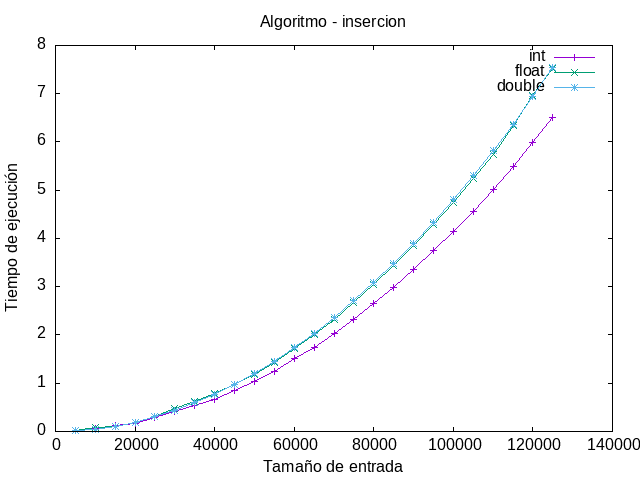
\includegraphics[width=\linewidth]{assets/Img/insercion.png}
        \caption{Ejecución algoritmo insercion}
        \label{fig:insercion}
    \end{minipage}%
    \begin{minipage}{0.5\textwidth}
        \centering
        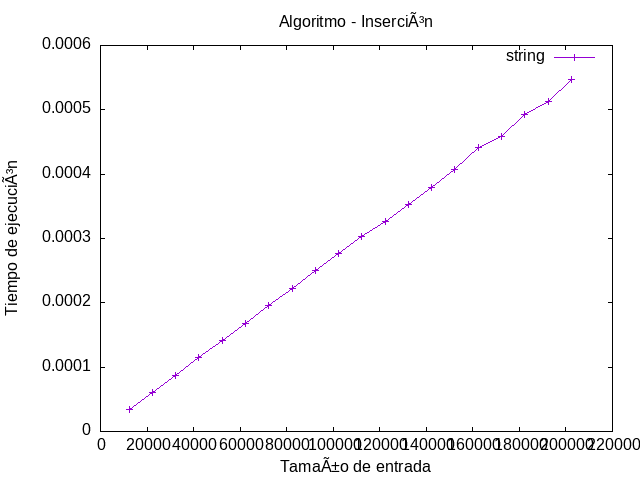
\includegraphics[width=\linewidth]{assets/Img/insercionstring.png}
        \caption{Ejecución algoritmo inserción con string}
        \label{fig:insercionstring}
    \end{minipage}
\end{figure}

\begin{table}[!ht]
    \centering
    \small
    \begin{tabular}{|l|l|l|l|l|l|l|l|}
    \hline
    \multicolumn{8}{|c|}{\cellcolor{blue!20}\textbf{Inserción}} \\ \hline
    \multicolumn{2}{|c|}{\cellcolor{gray!20}Tipo Int} & \multicolumn{2}{c|}{\cellcolor{gray!20}Tipo Float} & \multicolumn{2}{c|}{\cellcolor{gray!20}Tipo Double} & \multicolumn{2}{c|}{\cellcolor{gray!20}Tipo String}\\ \hline
        \textbf{Tamaño} & \textbf{Tiempo} & \textbf{Tamaño} & \textbf{Tiempo} & \textbf{Tamaño} & \textbf{Tiempo} & \textbf{Tamaño} & \textbf{Tiempo} \\ \hline
        5000 & 0,0202083 & 5000 & 0,0231026 & 5000 & 0,0123225 & 12308 & 3,45E-05 \\ \hline
        10000 & 0,0669288 & 10000 & 0,083436 & 10000 & 0,0489249 & 22308 & 6,10E-05 \\ \hline
        15000 & 0,118554 & 15000 & 0,109163 & 15000 & 0,10909 & 32308 & 8,77E-05 \\ \hline
        20000 & 0,171463 & 20000 & 0,194157 & 20000 & 0,194458 & 42308 & 0,000114708 \\ \hline
        25000 & 0,290236 & 25000 & 0,303104 & 25000 & 0,303342 & 52308 & 0,000141829 \\ \hline
        30000 & 0,4179 & 30000 & 0,474516 & 30000 & 0,437655 & 62308 & 0,000168388 \\ \hline
        35000 & 0,546578 & 35000 & 0,611683 & 35000 & 0,591596 & 72308 & 0,000195308 \\ \hline
        40000 & 0,664381 & 40000 & 0,788565 & 40000 & 0,772917 & 82308 & 0,000222477 \\ \hline
        45000 & 0,844561 & 45000 & 0,967047 & 45000 & 0,97772 & 92308 & 0,000249857 \\ \hline
        50000 & 1,03853 & 50000 & 1,1911 & 50000 & 1,20692 & 102308 & 0,000276907 \\ \hline
        55000 & 1,25102 & 55000 & 1,43977 & 55000 & 1,45909 & 112308 & 0,000303237 \\ \hline
        60000 & 1,51964 & 60000 & 1,71672 & 60000 & 1,73629 & 122308 & 0,000326027 \\ \hline
        65000 & 1,7472 & 65000 & 2,00781 & 65000 & 2,03246 & 132308 & 0,000353216 \\ \hline
        70000 & 2,03282 & 70000 & 2,32859 & 70000 & 2,35687 & 142308 & 0,000379146 \\ \hline
        75000 & 2,32695 & 75000 & 2,67209 & 75000 & 2,70622 & 152308 & 0,000406996 \\ \hline
        80000 & 2,64902 & 80000 & 3,04303 & 80000 & 3,0808 & 162308 & 0,000441945 \\ \hline
        85000 & 2,99459 & 85000 & 3,43543 & 85000 & 3,47801 & 172308 & 0,000459225 \\ \hline
        90000 & 3,35945 & 90000 & 3,8531 & 90000 & 3,90283 & 182308 & 0,000492385 \\ \hline
        95000 & 3,74271 & 95000 & 4,28721 & 95000 & 4,34073 & 192308 & 0,000513575 \\ \hline
        100000 & 4,14988 & 100000 & 4,75486 & 100000 & 4,81364 & 202308 & 0,000547894 \\ \hline
        105000 & 4,56802 & 105000 & 5,23354 & 105000 & 5,30147 & ~ & ~ \\ \hline
        110000 & 5,01684 & 110000 & 5,74715 & 110000 & 5,8236 & ~ & ~ \\ \hline
        115000 & 5,48697 & 115000 & 6,3353 & 115000 & 6,36572 & ~ & ~ \\ \hline
        120000 & 5,98221 & 120000 & 6,95729 & 120000 & 6,93946 & ~ & ~ \\ \hline
        125000 & 6,51173 & 125000 & 7,53129 & 125000 & 7,54045 & ~ & \\\hline
    \end{tabular}
\end{table}

\subsection*{Mergesort}
El algoritmo mergesort es del tipo $O(n\log(n))$ por tanto su tiempo de ejecución se ve reducido en comparación a los algoritmos 
anteriormente vistos, lso datos numéricos se coimportan de forma parecida en los tres casos.
\begin{figure}[H]
    \begin{minipage}{0.5\textwidth}
        \centering
        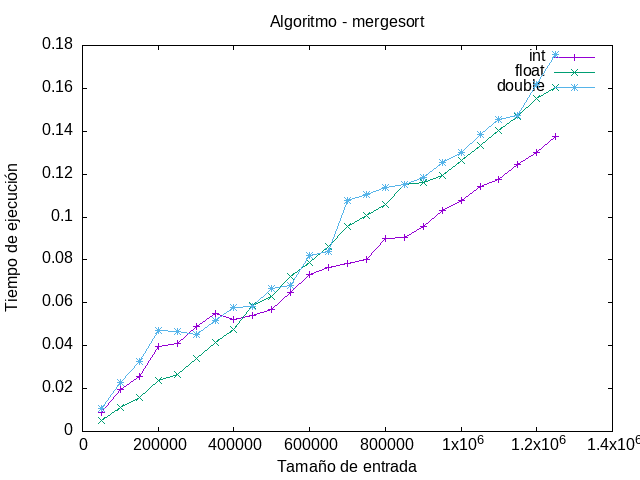
\includegraphics[width=\linewidth]{assets/Img/mergesort.png}
        \caption{Ejecución algoritmo Mergesort}
        \label{fig:mergesort}
    \end{minipage}%
    \begin{minipage}{0.5\textwidth}
        \centering
        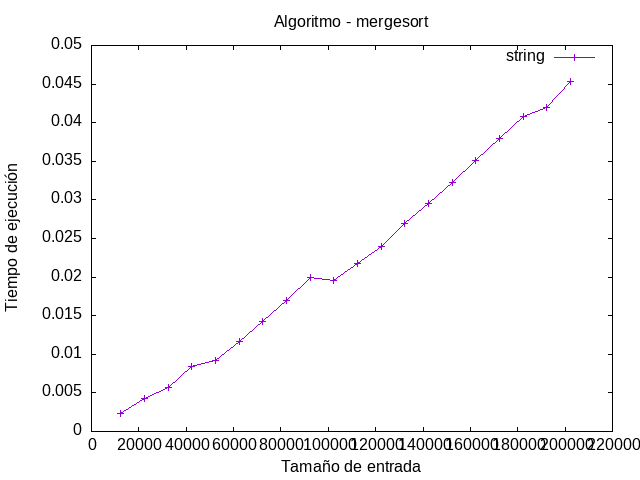
\includegraphics[width=\linewidth]{assets/Img/mergesortstring.png}
        \caption{Ejecución algoritmo Mergesort con string}
        \label{fig:mergesortstring}
    \end{minipage}
\end{figure}

\begin{table}[!ht]
    \centering
    \small
    \begin{tabular}{|l|l|l|l|l|l|l|l|}
    \hline
    \multicolumn{8}{|c|}{\cellcolor{blue!20}\textbf{Mergesort}} \\ \hline
    \multicolumn{2}{|c|}{\cellcolor{gray!20}Tipo Int} & \multicolumn{2}{c|}{\cellcolor{gray!20}Tipo Float} & \multicolumn{2}{c|}{\cellcolor{gray!20}Tipo Double} & \multicolumn{2}{c|}{\cellcolor{gray!20}Tipo String}\\ \hline
        \textbf{Tamaño} & \textbf{Tiempo} & \textbf{Tamaño} & \textbf{Tiempo} & \textbf{Tamaño} & \textbf{Tiempo} & \textbf{Tamaño} & \textbf{Tiempo} \\ \hline
        50000 & 0,00885563 & 50000 & 0,00535974 & 50000 & 0,0109506 & 12308 & 0,00232464 \\ \hline
        100000 & 0,0197725 & 100000 & 0,0113207 & 100000 & 0,0229505 & 22308 & 0,00426666 \\ \hline
        150000 & 0,0256754 & 150000 & 0,0159655 & 150000 & 0,032702 & 32308 & 0,00570479 \\ \hline
        200000 & 0,0396519 & 200000 & 0,0238364 & 200000 & 0,0470055 & 42308 & 0,00839818 \\ \hline
        250000 & 0,0408458 & 250000 & 0,0263662 & 250000 & 0,0465912 & 52308 & 0,00923186 \\ \hline
        300000 & 0,0487663 & 300000 & 0,0338221 & 300000 & 0,045297 & 62308 & 0,0115959 \\ \hline
        350000 & 0,0550213 & 350000 & 0,0412734 & 350000 & 0,0516928 & 72308 & 0,0142777 \\ \hline
        400000 & 0,0522138 & 400000 & 0,0473443 & 400000 & 0,0576073 & 82308 & 0,0169875 \\ \hline
        450000 & 0,0539998 & 450000 & 0,0587599 & 450000 & 0,0581018 & 92308 & 0,0199003 \\ \hline
        500000 & 0,0567018 & 500000 & 0,0631239 & 500000 & 0,0668968 & 102308 & 0,0195291 \\ \hline
        550000 & 0,0649299 & 550000 & 0,0721455 & 550000 & 0,0680914 & 112308 & 0,0217157 \\ \hline
        600000 & 0,0730137 & 600000 & 0,078831 & 600000 & 0,0821479 & 122308 & 0,0240279 \\ \hline
        650000 & 0,0765446 & 650000 & 0,0864586 & 650000 & 0,0840685 & 132308 & 0,0269058 \\ \hline
        700000 & 0,0783553 & 700000 & 0,095748 & 700000 & 0,107731 & 142308 & 0,0295147 \\ \hline
        750000 & 0,0801539 & 750000 & 0,1006187 & 750000 & 0,110418 & 152308 & 0,0322954 \\ \hline
        800000 & 0,0898059 & 800000 & 0,105794 & 800000 & 0,113999 & 162308 & 0,0350564 \\ \hline
        850000 & 0,0904214 & 850000 & 0,11503 & 850000 & 0,115276 & 172308 & 0,0379305 \\ \hline
        900000 & 0,0957652 & 900000 & 0,115988 & 900000 & 0,118358 & 182308 & 0,040835 \\ \hline
        950000 & 0,102922 & 950000 & 0,119324 & 950000 & 0,125308 & 192308 & 0,041929 \\ \hline
        1000000 & 0,10751 & 1000000 & 0,126549 & 1000000 & 0,130252 & 202308 & 0,0454001 \\ \hline
        1050000 & 0,114045 & 1050000 & 0,133461 & 1050000 & 0,138512 & ~ & ~ \\ \hline
        1100000 & 0,117457 & 1100000 & 0,140533 & 1100000 & 0,145543 & ~ & ~ \\ \hline
        1150000 & 0,124595 & 1150000 & 0,147092 & 1150000 & 0,147466 & ~ & ~ \\ \hline
        1200000 & 0,130175 & 1200000 & 0,155134 & 1200000 & 0,161852 & ~ & ~ \\ \hline
        1250000 & 0,137581 & 1250000 & 0,160264 & 1250000 & 0,175689 & ~ & \\\hline
    \end{tabular}
\end{table}
\subsection*{Quicksort}
El algoritmo quicksort es el último de los algoritmos de ordenación vistos en esta práctica , tiene eficiencia $O(n\log(n))$ y se comporta de 
forma parecida con los 3 tipos de datos numericos pero  a la hora de orenar strings aumenta su tiempo de ejecución debido a la existencia de datos repetidos 
en gran cantidad por tanto se comporta mas parecido a un algoritmo de eficiencia cuadrática que a uno de eficiencia logaritmica.
\begin{figure}[H]
    \begin{minipage}{0.5\textwidth}
        \centering
        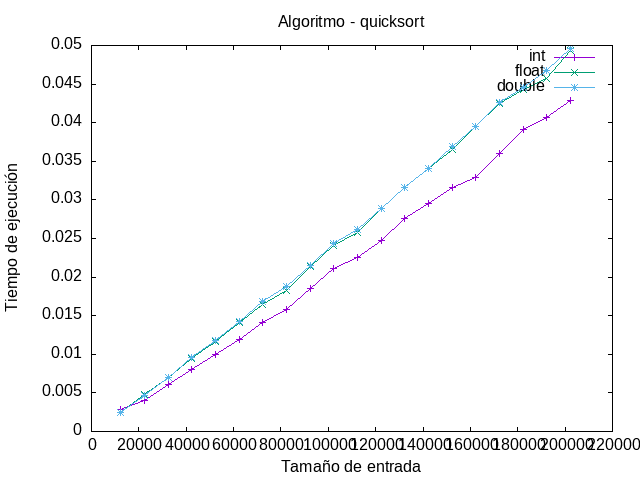
\includegraphics[width=\linewidth]{assets/Img/quicksort.png}
        \caption{Ejecución algoritmo quicksort}
        \label{fig:quicksort}
    \end{minipage}%
    \begin{minipage}{0.5\textwidth}
        \centering
        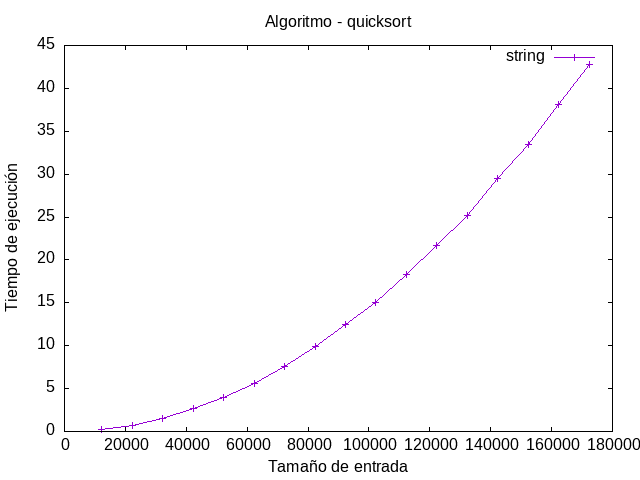
\includegraphics[width=\linewidth]{assets/Img/quicksortstring.png}
        \caption{Ejecución algoritmo quicksort con string}
        \label{fig:quicksortstring}
    \end{minipage}
\end{figure}

\begin{table}[!ht]
    \centering
    \small
    \begin{tabular}{|l|l|l|l|l|l|l|l|}
    \hline
    \multicolumn{8}{|c|}{\cellcolor{blue!20}\textbf{Quicksort}} \\ \hline
    \multicolumn{2}{|c|}{\cellcolor{gray!20}Tipo Int} & \multicolumn{2}{c|}{\cellcolor{gray!20}Tipo Float} & \multicolumn{2}{c|}{\cellcolor{gray!20}Tipo Double} & \multicolumn{2}{c|}{\cellcolor{gray!20}Tipo String}\\ \hline
        \textbf{Tamaño} & \textbf{Tiempo} & \textbf{Tamaño} & \textbf{Tiempo} & \textbf{Tamaño} & \textbf{Tiempo} & \textbf{Tamaño} & \textbf{Tiempo} \\ \hline
        50000 & 0,005404063 & 50000 & 0,00656497 & 50000 & 0,006872607 & 12308 & 0,331982 \\ \hline
        100000 & 0,011849567 & 100000 & 0,013940933 & 100000 & 0,014531567 & 22308 & 0,433525 \\ \hline
        150000 & 0,017589967 & 150000 & 0,021820767 & 150000 & 0,022618533 & 32308 & 0,810498 \\ \hline
        200000 & 0,0238955 & 200000 & 0,0290163 & 200000 & 0,030920433 & 42308 & 1,16745 \\ \hline
        250000 & 0,030245667 & 250000 & 0,036930167 & 250000 & 0,036553033 & 52308 & 1,97952 \\ \hline
        300000 & 0,035111167 & 300000 & 0,0380422 & 300000 & 0,039921433 & 62308 & 2,74097 \\ \hline
        350000 & 0,038264933 & 350000 & 0,038178767 & 350000 & 0,0424273 & 72308 & 3,55831 \\ \hline
        400000 & 0,0422403 & 400000 & 0,0424919 & 400000 & 0,043377433 & 82308 & 4,67599 \\ \hline
        450000 & 0,043866967 & 450000 & 0,0473254 & 450000 & 0,046259633 & 92308 & 5,73606 \\ \hline
        500000 & 0,04426 & 500000 & 0,048482467 & 500000 & 0,048961533 & 102308 & 7,04456 \\ \hline
        550000 & 0,048515033 & 550000 & 0,054502367 & 550000 & 0,052008133 & 112308 & 8,1903 \\ \hline
        600000 & 0,053473367 & 600000 & 0,0560969 & 600000 & 0,054563333 & 122308 & 10,0859 \\ \hline
        650000 & 0,058109467 & 650000 & 0,059735933 & 650000 & 0,055753933 & 132308 & 11,609 \\ \hline
        700000 & 0,061405633 & 700000 & 0,063045867 & 700000 & 0,058111633 & 142308 & 13,1231 \\ \hline
        750000 & 0,063922067 & 750000 & 0,0668639 & 750000 & 0,062652933 & 152308 & 15,4072 \\ \hline
        800000 & 0,065804867 & 800000 & 0,067741133 & 800000 & 0,066167833 & 162308 & 17,1388 \\ \hline
        850000 & 0,069073833 & 850000 & 0,073830267 & 850000 & 0,072807833 & 172308 & 19,0906 \\ \hline
        900000 & 0,073182433 & 900000 & 0,077997333 & 900000 & 0,0773843 & ~ & ~ \\ \hline
        950000 & 0,0761217 & 950000 & 0,081192567 & 950000 & 0,0808991 & ~ & ~ \\ \hline
        1000000 & 0,079173767 & 1000000 & 0,085758067 & 1000000 & 0,087570933 & ~ & ~ \\ \hline
        1050000 & 0,082858733 & 1050000 & 0,0920956 & 1050000 & 0,095611733 & ~ & ~ \\ \hline
        1100000 & 0,0841312 & 1100000 & 0,097475333 & 1100000 & 0,098788367 & ~ & ~ \\ \hline
        1150000 & 0,0922743 & 1150000 & 0,100609 & 1150000 & 0,100115767 & ~ & ~ \\ \hline
        1200000 & 0,095589967 & 1200000 & 0,104688333 & 1200000 & 0,103156333 & ~ & ~ \\ \hline
        1250000 & 0,096988633 & 1250000 & 0,109222 & 1250000 & 0,10996 & ~ & \\\hline
    \end{tabular}
\end{table}

\subsection*{Hanoi}
Este algoritmo es del orden $O(2^n)$ , se puede observar que a partir de un tamaño superior a 30 el tiempo de ejecución se ve 
altamente afectado.
\begin{figure}[H]
    \begin{minipage}{0.5\textwidth}
        \centering
        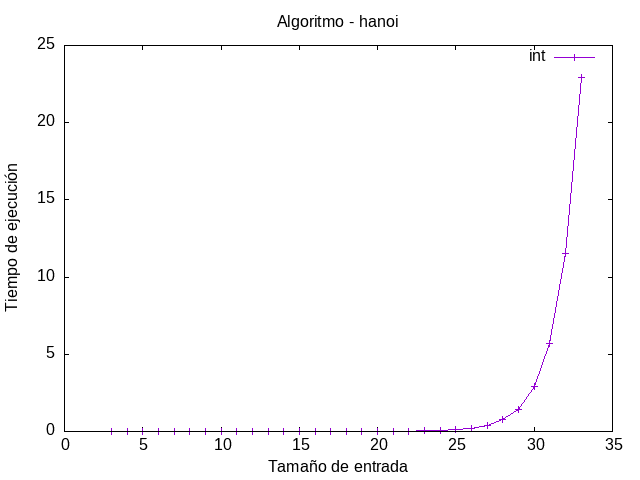
\includegraphics[width=\linewidth]{assets/Img/hanoiint.png}
        \caption{Ejecución algoritmo Hanoi}
        \label{fig:hanoi} 
    \end{minipage}%
    \begin{minipage}{0.5\textwidth}
        \centering
        \small
        \begin{tabular}{|l|l|l|l|}
        \hline
            \multicolumn{4}{|c|}{\cellcolor{blue!20}\textbf{Hanoi}} \\ \hline 
            \textbf{Tamaño} & \textbf{Tiempo} & \textbf{Tamaño} & \textbf{Tiempo} \\ \hline
            3 & 3.3e-07 & 19 & 0.00283343 \\ \hline
            4 & 3.7e-07 & 20 & 0.00583306 \\ \hline
            5 & 6.4e-07 & 21 & 0.0113207 \\ \hline
            6 & 9.1e-07 & 22 & 0.023259 \\ \hline
            7 & 1.31e-06 & 23 & 0.04468322 \\ \hline
            8 & 2.13e-06 & 24 & 0.0678575 \\ \hline
            9 & 0,003659 & 25 & 0.115696 \\ \hline
            10 & 0,006809 & 26 & 0.205652 \\ \hline
            11 & 9.15e-06 & 27 & 0.387235 \\ \hline
            12 & 0,02484 & 28 & 0.757241 \\ \hline
            13 & 0,43039 & 29 & 1.45715 \\ \hline
            14 & 0,91049 & 30 & 2.91489 \\ \hline
            15 & 0.000180597 & 31 & 5.73008 \\ \hline
            16 & 0.000370175 & 32 & 11.5402 \\ \hline
            17 & 0.000728411 & 33 & 22.9485 \\ \hline
            18 & 0.00143246 & ~ & \\ \hline
        \end{tabular}
    \end{minipage}
\end{figure}

\subsection*{Fibonacci}
El algoritmo de Fibonnaci es del orden $O((\frac{1+\sqrt{5}}{2})^n)$ y por tanto su compiortamiento es parecido al del algoritmo Hanoi ya que se puede
observar que a partir de cierto tamaño de entrada , en este caso 42 el tiempo de ejecución comienza a aumentar.
\begin{figure}[H]
    \begin{minipage}{0.5\textwidth}
        \centering
        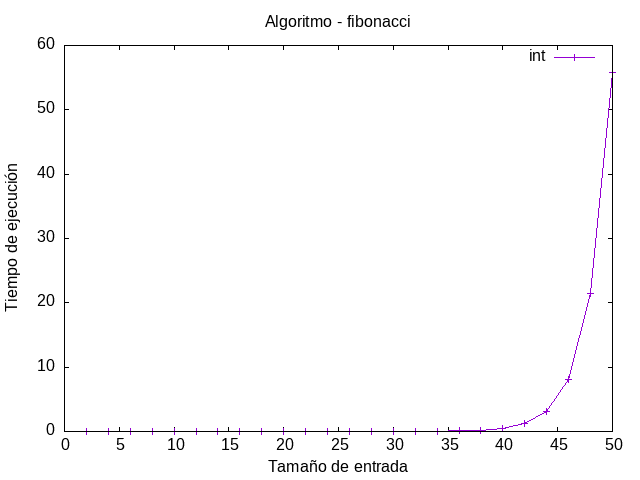
\includegraphics[width=\linewidth]{assets/Img/fibonacciint.png}
        \caption{Ejecución algoritmo Fibonacci}
        \label{fig:fibonacci}
    \end{minipage}%
    \begin{minipage}{0.5\textwidth}
        \centering
        \small
        \begin{tabular}{|l|l|l|l|}
        \hline
        \multicolumn{4}{|c|}{\cellcolor{blue!20}\textbf{Fibonacci}} \\ \hline 
        \textbf{Tamaño} & \textbf{Tiempo} & \textbf{Tamaño} & \textbf{Tiempo} \\ \hline
        2 & 1,90E-07 & 28 & 0,00269092 \\ \hline
        4 & 2,50E-07 & 30 & 0,00702187 \\ \hline
        6 & 3,10E-07 & 32 & 0,0188891 \\ \hline
        8 & 6,20E-07 & 34 & 0,0493608 \\ \hline
        10 & 1,13E-06 & 36 & 0,101751 \\ \hline
        12 & 2,11E-06 & 38 & 0,173823 \\ \hline
        14 & 4,42E-06 & 40 & 0,466558 \\ \hline
        16 & 9,70E-06 & 42 & 1,23353 \\ \hline
        18 & 2,34E-05 & 44 & 3,14718 \\ \hline
        20 & 5,86E-05 & 46 & 8,09745 \\ \hline
        22 & 0,000155419 & 48 & 21,4575 \\ \hline
        24 & 0,000392447 & 50 & 55,7656 \\ \hline
        26 & 0,00103918 & ~ & \\ \hline
        \end{tabular}
    \end{minipage}
\end{figure}

\subsection*{Floyd}
El último algoritmo es del orden $O(n^3)$ y su ejecución es parecida a los de orden $O(n^2)$ viendo que a partir de una entrada mayor a 
600 empieza a aumentar el tiempo de manera considerable.
\begin{figure}[H]
    \begin{minipage}{0.5\textwidth}
        \centering
        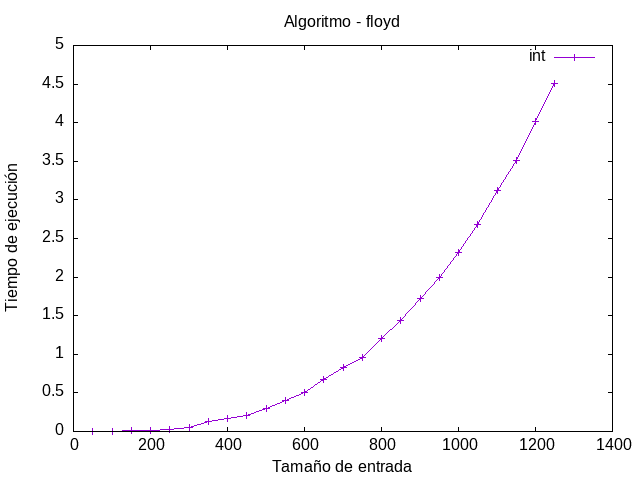
\includegraphics[width=\linewidth]{assets/Img/floydint.png}
        \caption{Ejecución algoritmo Floyd}
        \label{fig:floyd}
    \end{minipage}
    \begin{minipage}{0.5\textwidth}
        \centering
        \small
        \begin{tabular}{|l|l|l|l|}
        \hline
        \multicolumn{4}{|c|}{\cellcolor{blue!20}\textbf{Floyd}} \\ \hline 
        \textbf{Tamaño} & \textbf{Tiempo} & \textbf{Tamaño} & \textbf{Tiempo} \\ \hline
        50 & 0,000317337 & 700 & 0,824563 \\ \hline
        100 & 0,00221242 & 750 & 0,956399 \\ \hline
        150 & 0,006823 & 800 & 1,19819 \\ \hline
        200 & 0,0089683 & 850 & 1,4429 \\ \hline
        250 & 0,0301016 & 900 & 1,71932 \\ \hline
        300 & 0,0513097 & 950 & 1,99518 \\ \hline
        350 & 0,133839 & 1000 & 2,31279 \\ \hline
        400 & 0,174386 & 1050 & 2,67816 \\ \hline
        450 & 0,207949 & 1100 & 3,11671 \\ \hline
        500 & 0,297192 & 1150 & 3,51038 \\ \hline
        550 & 0,399401 & 1200 & 4,01139 \\ \hline
        600 & 0,509953 & 1250 & 4,50535 \\ \hline
        650 & 0,667422 & ~ & \\ \hline
        \end{tabular}
    \end{minipage}
\end{figure}

\subsection{Ejecución en distintos ordenadores}
Finalmente, acabamos mostrando una comparación entre distintos ordenadores para el mismo algoritmo, para mostrar que cuando
el algoritmo es el mismo, la diferencia entre los tiempos de ejecución en distintos ordenadores será puramente de una constate, 
y el orden de eficiencia se mantendrá. En este caso, ejecutamos el algoritmo de inserción para los tipos de datos int y double, estos
fueron los resultados:
% Dos figuras centradas separadas
\begin{figure}[H]
    \begin{minipage}{0.5\textwidth}
        \centering
        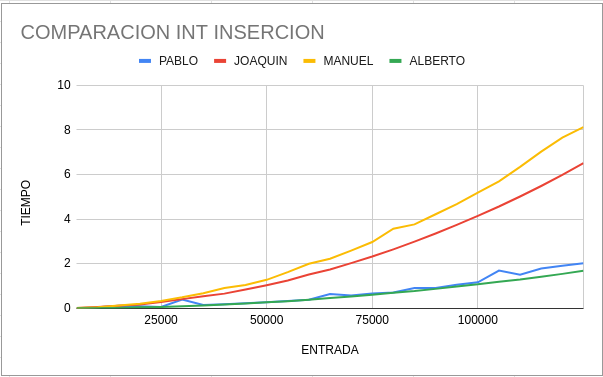
\includegraphics[width=\linewidth]{assets/Img/insercionordenadores.png}
        \caption{Ejecución algoritmo Inserción con Int}
        \label{fig:fibonacci}
    \end{minipage}
    \begin{minipage}{0.5\textwidth}
        \centering
        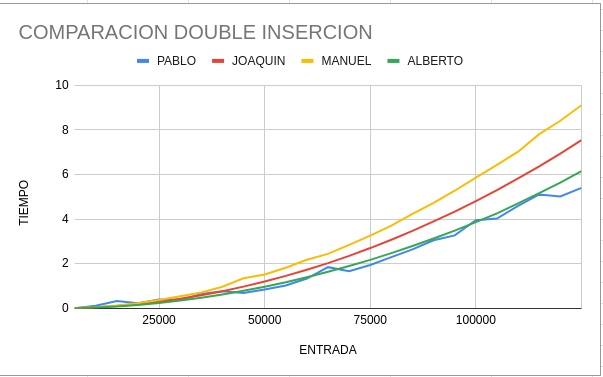
\includegraphics[width=\linewidth]{assets/Img/insercionordenadoresd.png}
        \caption{Ejecución algoritmo Insercion con Double}
    \end{minipage}
\end{figure}



\subsection{Estudio híbrido}
En esta sección, a partir del estudio híbrido, podremos observar como los datos obtenidos de forma \\
empírica, concuerdan con los resultados que deberiamos obtener de forma teorica.
\subsection*{Burbuja}
\begin{figure}[H]
    \begin{minipage}{0.5\textwidth}
        \centering
        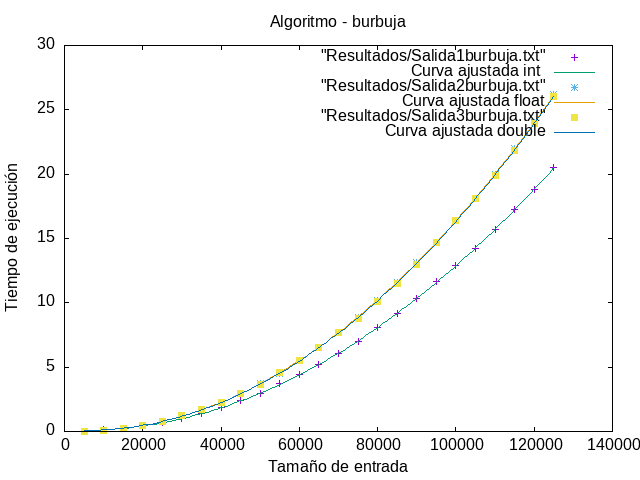
\includegraphics[width=\linewidth]{assets/AjusteHibrido_latex/Hibridoburbuja/burbuja_hib.png}
        \caption{Ajuste híbrido algoritmo burbuja}
        \label{fig:burbuja}
    \end{minipage}%
    \begin{minipage}{0.5\textwidth}
        \centering
        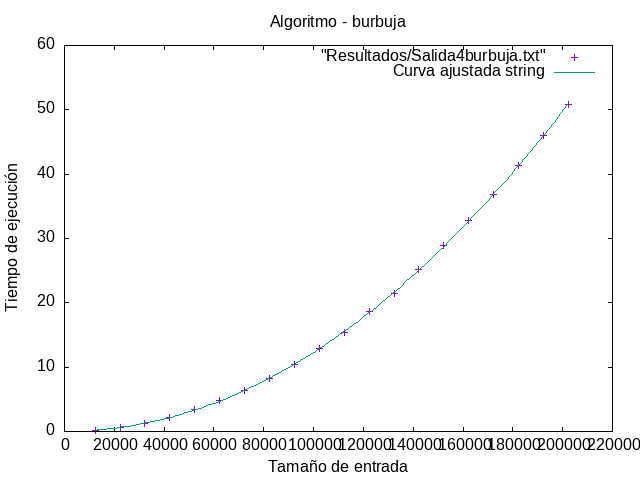
\includegraphics[width=\linewidth]{assets/AjusteHibrido_latex/Hibridoburbuja/burbujastring_hib.png}
        \caption{Ajuste híbrido algoritmo burbuja con string}
        \label{fig:burbujastring}
    \end{minipage}
\end{figure}
Tras la interpretación de los datos empíricos en gnuplot y de la formula teorica del método, obtenemos que \\
las constantes ocultas son:
\begin{align*}
    T_{burbujaInt}(n) &=1.41315 \cdot 10^{-9}x^{2}-1.3691 \cdot 10^{-5}x+0.127228 \\
    T_{burbujaFloat}(n) &=1.82299 \cdot 10^{-9}x^{2}-1.98111 \cdot 10^{-5}x+0.134867 \\
    T_{burbujaDouble}(n) &=1.82075 \cdot 10^{-9}x^{2}-2.20296 \cdot 10^{-5}x+0.144178 \\
    T_{burbujaString}(n) &=1.26281 \cdot 10^{-9}x^{2}-4.03916 \cdot 10^{-5}x+0.0834222 
\end{align*}


También podemos ver la varianza en la calidad del ajuste. 
\begin{align*}
    V_{burbujaInt}&=0.000944698 \\
    V_{burbujaFloat}&=0.000528375 \\
    V_{burbujaDouble}&=0.00199636 \\
    V_{burbujaString}&=0.00645483
\end{align*}

\subsection*{Selección}
\begin{figure}[H]
    \begin{minipage}{0.5\textwidth}
        \centering
        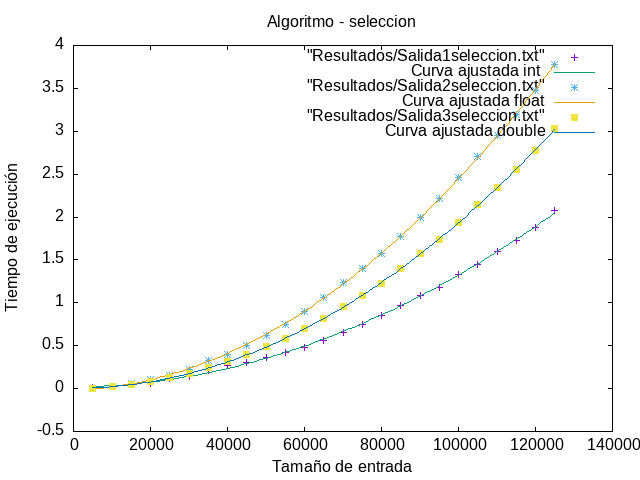
\includegraphics[width=\linewidth]{assets/AjusteHibrido_latex/Hibridoseleccion/seleccion_hib.png}
        \caption{Ajuste híbrido algoritmo selección}
        \label{fig:seleccion}
    \end{minipage}%
    \begin{minipage}{0.5\textwidth}
        \centering
        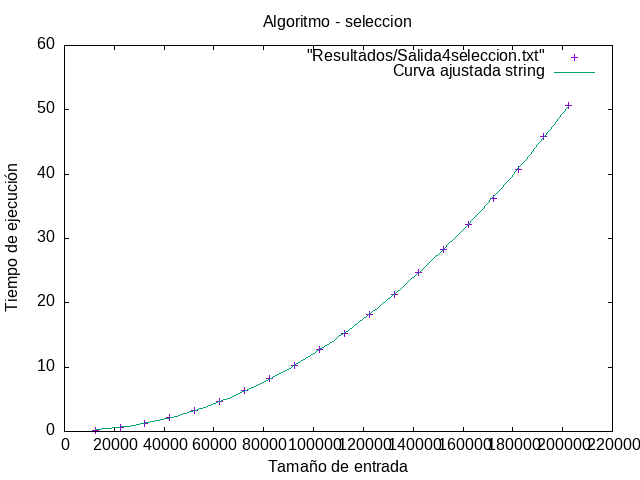
\includegraphics[width=\linewidth]{assets/AjusteHibrido_latex/Hibridoseleccion/seleccionstring_hib.png}
        \caption{Ajuste híbrido algoritmo seleccion con string}
        \label{fig:Seleccion}
    \end{minipage}
\end{figure}
Tras la interpretación de los datos empíricos en gnuplot y de la formula teorica del métoco, obtenemos que \\
las constantes ocultas son:
\begin{align*}
        T_{\text{SelecciónInt}}(n)&=1.2734 \cdot 10^{-10}x^{2}+3.1274 \cdot 10^{-7}x+0.018826 \\
        T_{\text{SelecciónFloat}}(n)&=2.31309 \cdot 10^{-9}x^{2}+1.4781 \cdot 10^{-6}x-0.0183413 \\
        T_{\text{SelecciónDouble}}(n)&=1.94045 \cdot 10^{-10}x^{2}-1.00224 \cdot 10^{-7}x+0.00447121 \\
        T_{\text{SelecciónString}}(n)&=1.27216 \cdot 10^{-9}x^{2}-8.8078 \cdot 10^{-6}x+0.233527 
\end{align*}

También podemos ver la varianza en la calidad del ajuste. 
\begin{align*}
    V_{seleccionInt}&=0.00026937 \\
    V_{seleccionFloat}&=0.000114947 \\
    V_{seleccionDouble}&=3.49475 \cdot 10^{-5} \\
    V_{seleccionString}&=0.0160175
\end{align*}
\subsection*{Inserción}
\begin{figure}[H]
    \begin{minipage}{0.5\textwidth}
        \centering
        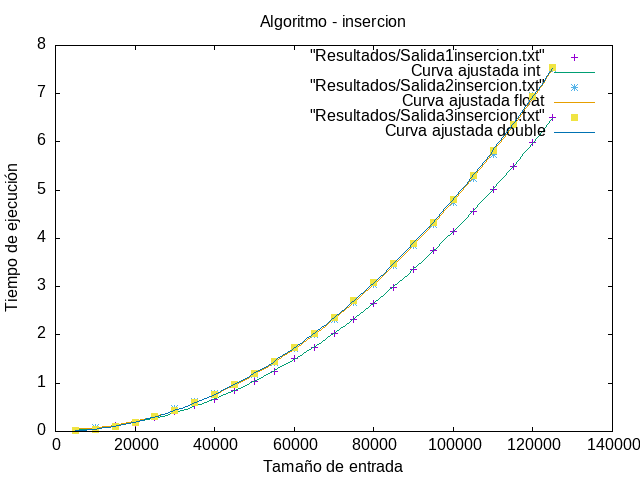
\includegraphics[width=\linewidth]{assets/AjusteHibrido_latex/Hibridoinsercion/insercion_hib.png}
        \caption{Ajuste híbrido algoritmo inserción}
        \label{fig:insercion}
    \end{minipage}%
    \begin{minipage}{0.5\textwidth}
        \centering
        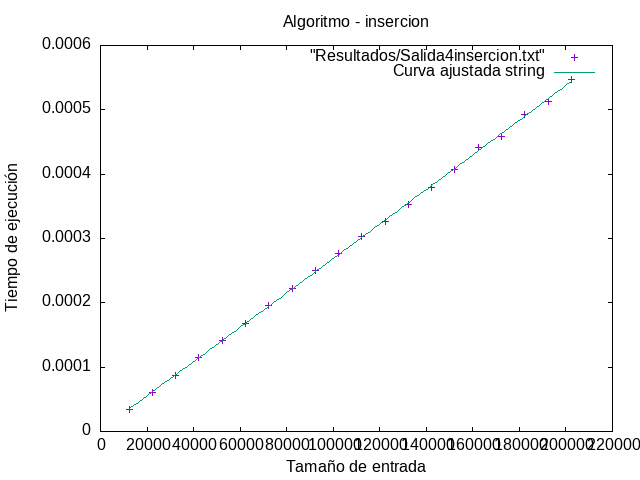
\includegraphics[width=\linewidth]{assets/AjusteHibrido_latex/Hibridoinsercion/insercionstring_hib.png}
        \caption{Ajuste híbrido algoritmo inserción con string}
        \label{fig:insercion}
    \end{minipage}
\end{figure}
Tras la interpretación de los datos empíricos en gnuplot y de la formula teorica del métoco, obtenemos que \\
las constantes ocultas son:
\begin{align*}
    T_{inserciónInt}(n)&=4.19645 \cdot 10^{-10}x^{2}-8.0708 \cdot 10^{-7}x+0.0346585 \\
    T_{inserciónFloat}(n)&=4.91154 \cdot 10^{-10}x^{2}-1.81363 \cdot 10^{-6}x-0.0478225 \\
    T_{inserciónDouble}(n)&=4.82763 \cdot 10^{-10}x^{2}-1.65187 \cdot 10^{-7}x+0.00477564 \\
    T_{inserciónString}(n)&=1.56549 \cdot 10^{-16}x^{2}+2.64624 \cdot 10^{-9}x+2.52872 \cdot 10^{-6}
\end{align*}
También podemos ver la varianza en la calidad del ajuste. 
\begin{align*}
    V_{\text{InserciónInt}}&=0.000177503 \\
    V_{\text{InserciónFloat}}&=0.0000614231 \\
    V_{\text{InserciónDouble}}&=1.92651 \cdot 10^{-5} \\
    V_{\text{InserciónString}}&=6.94094\cdot 10^{-12}
\end{align*}

\subsection*{Mergesort}
\begin{figure}[H]
    \begin{minipage}{0.5\textwidth}
        \centering
        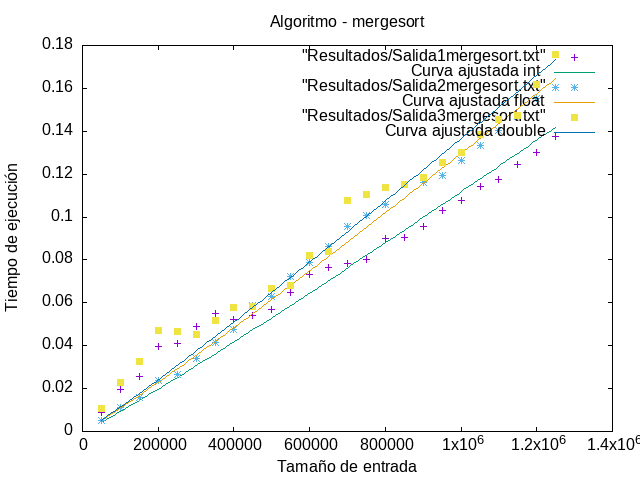
\includegraphics[width=\linewidth]{assets/AjusteHibrido_latex/Hibridomergesort/mergesort_hib.png}
        \caption{Ajuste híbrido algoritmo mergesort}
        \label{fig:mergesort}
    \end{minipage}%
    \begin{minipage}{0.5\textwidth}
        \centering
        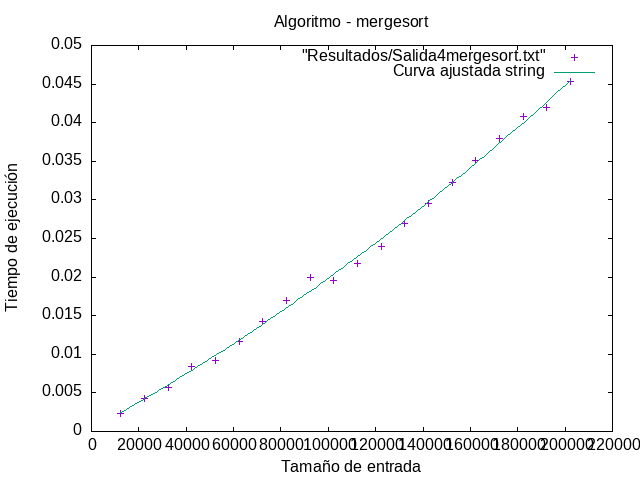
\includegraphics[width=\linewidth]{assets/AjusteHibrido_latex/Hibridomergesort/mergesortstring_hib.png}
        \caption{Ajuste híbrido algoritmo mergesort con string}
        \label{fig:mergesort}
    \end{minipage}
\end{figure}
Tras la interpretación de los datos empíricos en gnuplot y de la formula teorica del métoco, obtenemos que \\
las constantes ocultas son:
\begin{equation*}
    T_{mergesortInt}=8.0872\cdot 10^{-9}x log(x)
\end{equation*}
\begin{equation*}
    T_{mergesortFloat}=9.38225\cdot 10^{-9}x log(x)
\end{equation*}
\begin{equation*}
    T_{mergesortDouble}=9.88488\cdot 10^{-9}x log(x)
\end{equation*}
\begin{equation*}
    T_{mergesortrString}=2.72414 \cdot 10^{-13}x^{2}+1.67908 \cdot 10^{-7}x+0.000330868 
\end{equation*}

También podemos ver la varianza en la calidad del ajuste. 
\begin{equation*}
    V_{mergesortInt}=8.73646\cdot 10^{-5}
\end{equation*}
\begin{equation*}
    V_{mergesortFloat}=1.2413\cdot 10^{-5}
\end{equation*}
\begin{equation*}
    V_{mergesortDouble}=8.32396 \cdot 10^{-5}
\end{equation*}
\begin{equation*}
    V_{mergesortrString}=5.46779 \cdot 10^{-7}
\end{equation*}
\\
Aquí, podemos observar como las gráficas para los datos numéricos concuerdan tanto su estudio teórico como 
empírico. Sin embargo, en el caso de la gráfica del tipo string la función que mejor se ajusta a los datos
obtenidos de forma empírica es la funcion 
\begin{equation*}
    f(x)=a_0 \cdot x^{2} + a_1 x + a_0
\end{equation*}

\subsection*{Quicksort}
\begin{figure}[H]
    \begin{minipage}{0.5\textwidth}
        \centering
        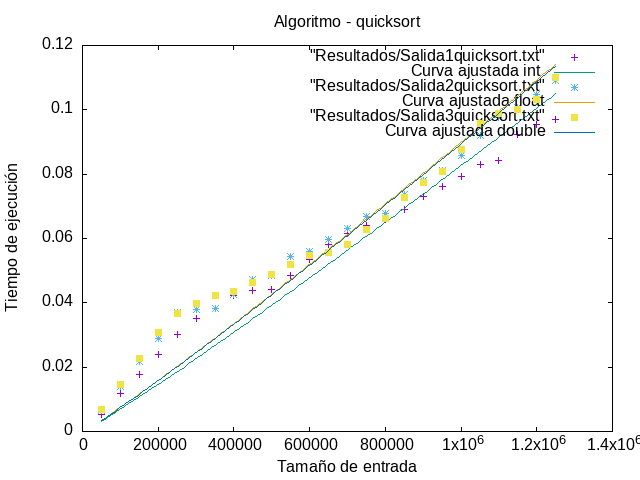
\includegraphics[width=\linewidth]{assets/AjusteHibrido_latex/Hibridoquicksort/quicksort_hib.png}
        \caption{Ajuste híbrido algoritmo quicksort}
        \label{fig:quicksort}
    \end{minipage}%
    \begin{minipage}{0.5\textwidth}
        \centering
        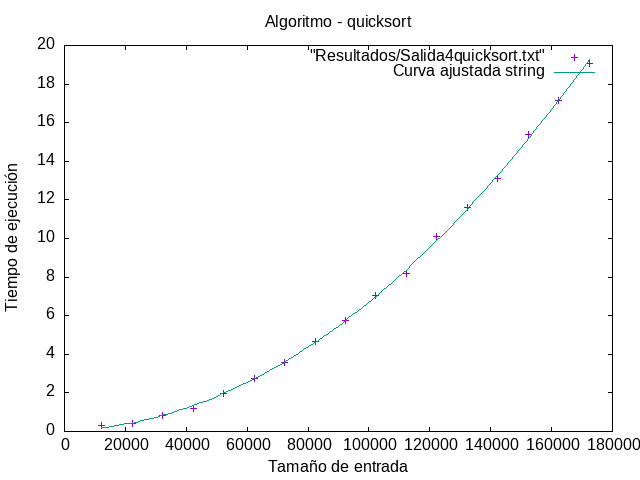
\includegraphics[width=\linewidth]{assets/AjusteHibrido_latex/Hibridoquicksort/quicksortstring_hib.png}
        \caption{Ajuste híbrido algoritmo quicksort con string}
        \label{fig:quicksort}
    \end{minipage}
\end{figure}
Tras la interpretación de los datos empíricos en gnuplot y de la formula teorica del métoco, obtenemos que \\
las constantes ocultas son:
\begin{align*}
    T_{quicksortInt}(n)&=5.98183\cdot 10^{-9}x log(x) \\
    T_{quicksortFloat}(n)&=6.50446\cdot 10^{-9}x log(x) \\
    T_{quicksortDouble}(n)&=6.47155\cdot 10^{-9}x log(x) \\
    T_{quicksortrString}(n)&=6.21508 \cdot 10^{-10}x^{2}+4.51207 \cdot 10^{-6}x+0.0387326
\end{align*}
También podemos ver la varianza en la calidad del ajuste. 
\begin{align*}
    V_{quicksortInt}&=4.76198\cdot 10^{-5} \\
    V_{quicksortFloat}&=5.29642\cdot 10^{-5} \\
    V_{quicksortDouble}&=6.13293 \cdot 10^{-5} \\
    V_{quicksortrString}&=0.0191243
\end{align*}
Como podemos ver, con este método ocurre lo mismo que con el mergesort. De este modo, tenemos que el ajuste híbrido
para las graficas de tipo numérico, se realiza con la formula obtenida en su estudio teórico. Mientras que en el tipo
string la fórmula que mejor se ajusta a los datos obtenidos empíricamente es
\begin{equation*}
    f(x)=a_0 \cdot x^{2} + a_1 x + a_0
\end{equation*}

\subsection*{Floyd, Fibonacci y Hanoi}
\begin{figure}[H]
    \begin{minipage}{0.5\textwidth}
        \centering
        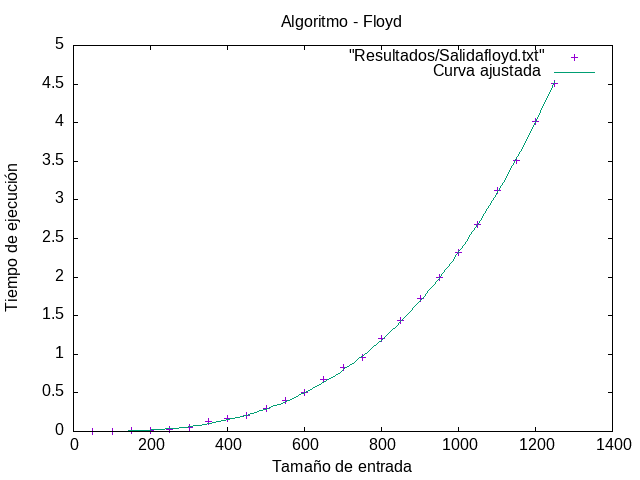
\includegraphics[width=\linewidth]{assets/AjusteHibrido_latex/Hibrido_fibonacci_floyd_hanoi/Floyd_hib.png}
        \caption{Ajuste híbrido floyd}
        \label{fig:floyd}
    \end{minipage}%
    \begin{minipage}{0.5\textwidth}
        \centering
        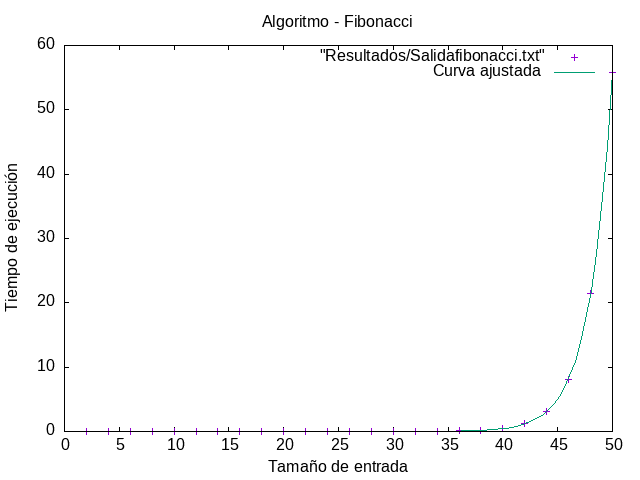
\includegraphics[width=\linewidth]{assets/AjusteHibrido_latex/Hibrido_fibonacci_floyd_hanoi/Fibonacci_hib.png}
        \caption{Ajuste híbrido fibonacci}
        \label{fig:fibonacci}
    \end{minipage}
    \begin{center}
        \begin{minipage}{0.5\textwidth}
            \centering
            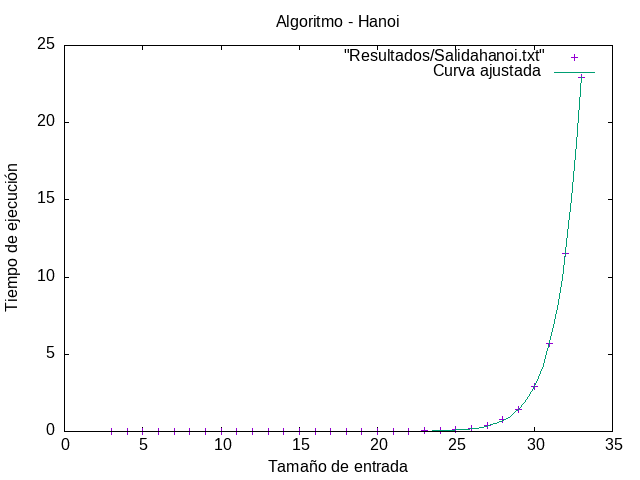
\includegraphics[width=\linewidth]{assets/AjusteHibrido_latex/Hibrido_fibonacci_floyd_hanoi/Hanoi_hib.png}
            \caption{Ajuste híbrido hanoi}
            \label{fig:hanoi}
        \end{minipage}
    \end{center}
\end{figure}
Tras la interpretación de los datos empíricos en gnuplot y de la formula teorica del métoco, obtenemos que \\
las constantes ocultas son:
\begin{align*}
    T_{Floyd}(n)&=2.32043\cdot 10^{-9}x^{3} \\
    T_{Fibonacci}(n)&=1.98321\cdot 10^{-9} \left(\frac{1+\sqrt{5}}{2}\right)^{x} \\
    T_{Hanoi}(n)&=2.67509\cdot 10^{-9} \cdot 2^{x}
\end{align*}


También podemos ver la varianza en la calidad del ajuste. 
\begin{equation*}
    V_{Floyd}=0.000328165
\end{equation*}
\begin{equation*}
    V_{Fibonacci}=0.00121339
\end{equation*}
\begin{equation*}
    V_{Hanoi}=0.000361913
\end{equation*}

\subsection{Ajustes incorrectos}
\begin{figure}[H]
    \begin{minipage}{0.5\textwidth}
        \centering
        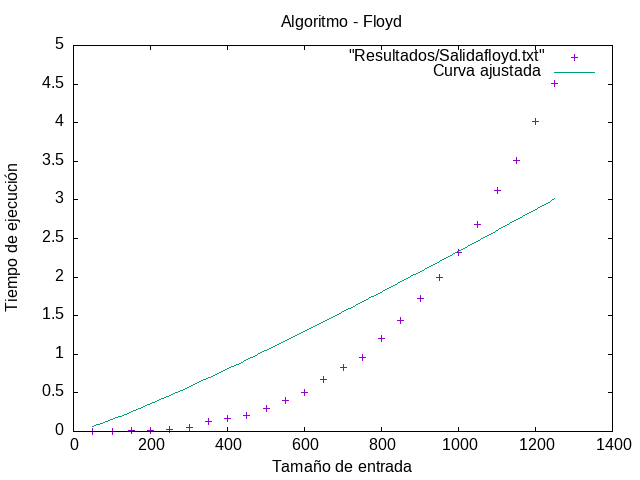
\includegraphics[width=\linewidth]{assets/AjusteIncorrecto/Floyd_hib.png}
        \caption{Ajuste incorrecto algoritmo floyd}
        \label{fig:floyd}
    \end{minipage}%
    \begin{minipage}{0.5\textwidth}
        \centering
        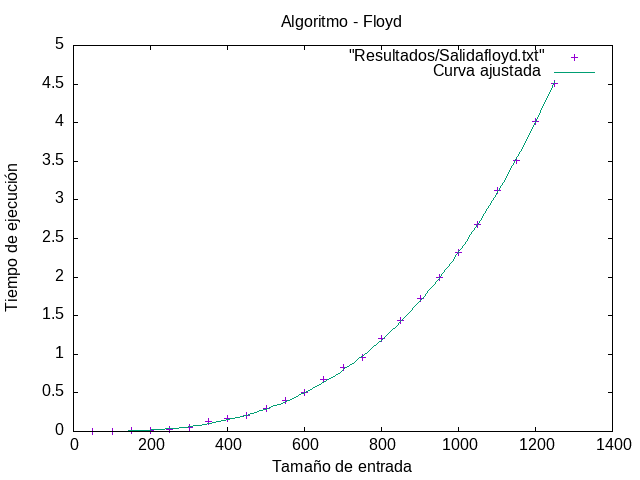
\includegraphics[width=\linewidth]{assets/AjusteHibrido_latex/Hibrido_fibonacci_floyd_hanoi/Floyd_hib.png}
        \caption{Ajuste correcto algoritmo floyd}
        \label{fig:floyd}
    \end{minipage}
\end{figure}
En la primera gráfica hemos utilizado la funcion $f(x)=a_0 \cdot xlog(x)$ para ajustar el método de 
Floyd. Como se puede observar,la función que mejor se ajusta al método de Floyd es la obtenida 
en el estudio teórico. Además, si comparamos sus varianzas podemos encontrar una diferencia de 
gran importancia
\begin{equation*}
    V_{FloydIncorrecto}=0.438352
\end{equation*}
\begin{equation*}
    V_{FloydCorrecto}=0.000328165
\end{equation*}

\begin{figure}[H]
    \begin{minipage}{0.5\textwidth}
        \centering
        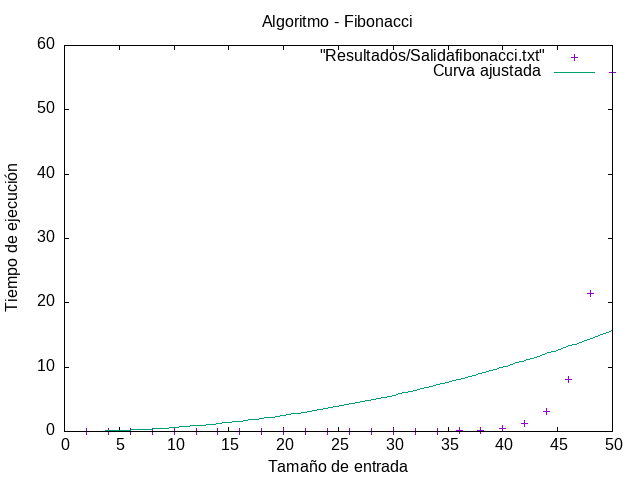
\includegraphics[width=\linewidth]{assets/AjusteIncorrecto/Fibonacci_hib.png}
        \caption{Ajuste incorrecto algoritmo fibonacci}
        \label{fig:fibonacci}
    \end{minipage}%
    \begin{minipage}{0.5\textwidth}
        \centering
        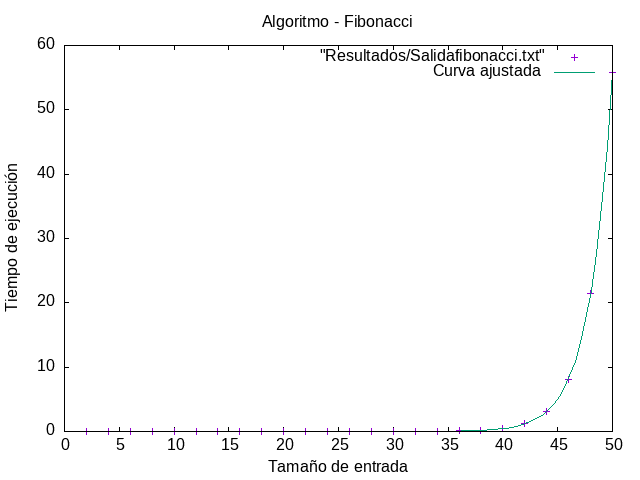
\includegraphics[width=\linewidth]{assets/AjusteHibrido_latex/Hibrido_fibonacci_floyd_hanoi/Fibonacci_hib.png}
        \caption{Ajuste correcto algoritmo fibonacci}
        \label{fig:fibonacci}
    \end{minipage}
\end{figure}
En la primera gráfica hemos utilizado la funcion $f(x)=a_0 \cdot x^{2}$ para ajustar el método de 
Fibonacci. Como se puede observar,la función que mejor se ajusta al método de Fibonacci es la obtenida 
en el estudio teórico. Además, si comparamos sus varianzas podemos encontrar una gran diferencia
\begin{equation*}
    V_{FibonacciIncorrecto}=95.8388
\end{equation*}
\begin{equation*}
    V_{FibonacciCorrecto}=0.00121339
\end{equation*}




\section{Estudio de las gráficas}
    En esta sección se mostrarán las gráficas obtenidas en el estudio empírico de los algoritmos. 
    \subsection{Algoritmos  \(O(n^2)\)}
    Comenzaremos comparando las gráficas obtenidas para los algoritmos de ordenación con eficiencia \(O(n^2)\)
    \begin{figure}[H]
        \begin{minipage}{0.5\textwidth}
            \centering
            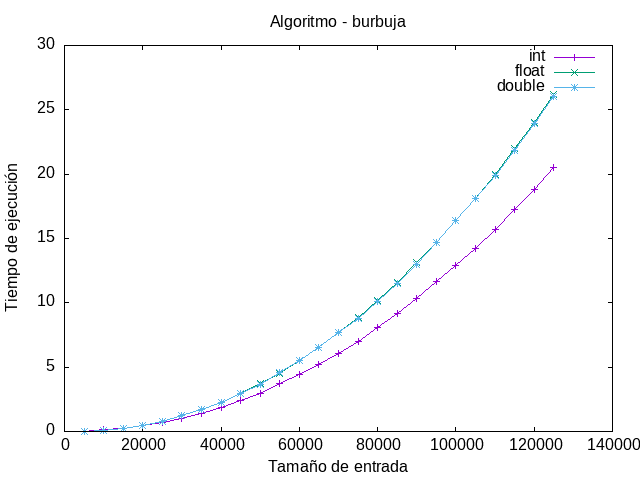
\includegraphics[width=\linewidth]{assets/Img/burbuja.png}
            \caption{Ejecución algoritmo burbuja}
            \label{fig:burbuja}
        \end{minipage}%
        \begin{minipage}{0.5\textwidth}
            \centering
            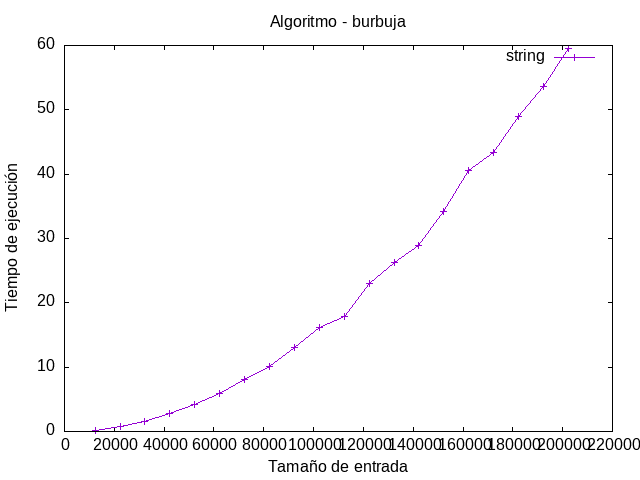
\includegraphics[width=\linewidth]{assets/Img/burbujastring.png}
            \caption{Ejecución algoritmo burbuja con string}
            \label{fig:burbujastring}
        \end{minipage}
    \end{figure}
    \begin{figure}[H]
        \begin{minipage}{0.5\textwidth}
            \centering
            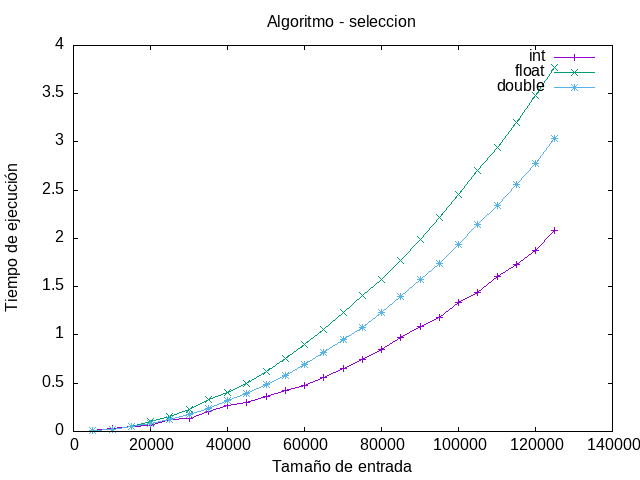
\includegraphics[width=\linewidth]{assets/Img/seleccion.png}
            \caption{Ejecución algoritmo seleccion}
            \label{fig:seleccion}
        \end{minipage}%
        \begin{minipage}{0.5\textwidth}
            \centering
            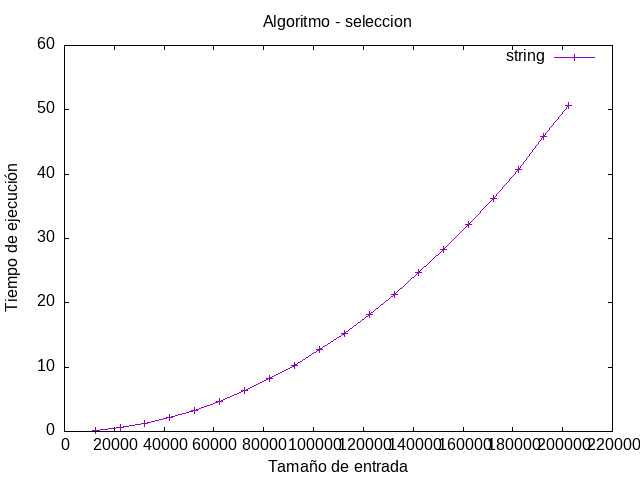
\includegraphics[width=\linewidth]{assets/Img/seleccionstring.png}
            \caption{Ejecución algoritmo seleccion con string}
            \label{fig:seleccionstring}
        \end{minipage}
    \end{figure}
    \begin{figure}[H]
        \begin{minipage}{0.5\textwidth}
            \centering
            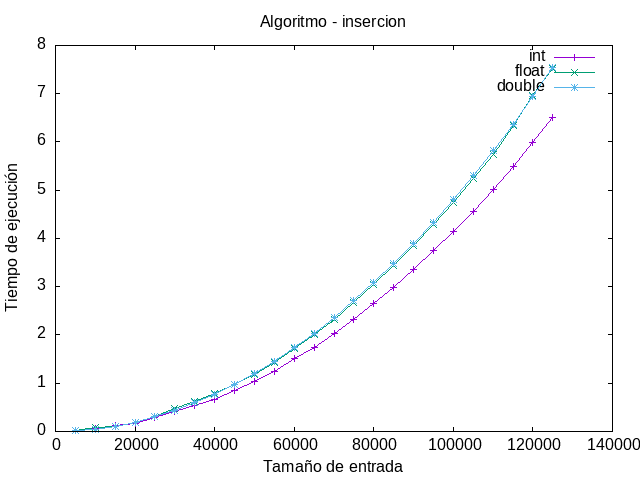
\includegraphics[width=\linewidth]{assets/Img/insercion.png}
            \caption{Ejecución algoritmo insercion}
            \label{fig:insercion}
        \end{minipage}%
        \begin{minipage}{0.5\textwidth}
            \centering
            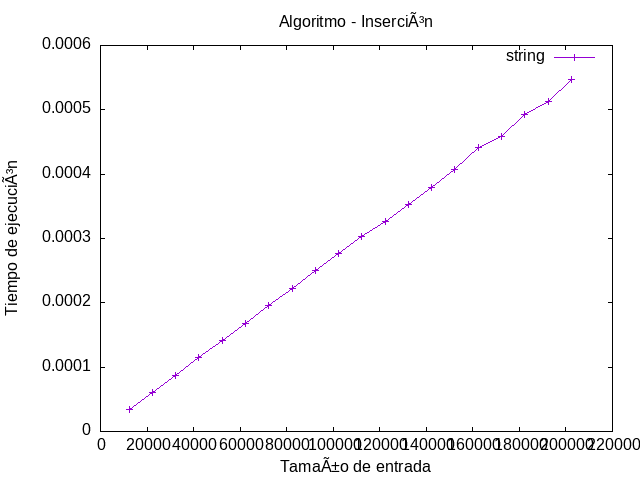
\includegraphics[width=\linewidth]{assets/Img/insercionstring.png}
            \caption{Ejecución algoritmo inserción con string}
            \label{fig:insercionstring}
        \end{minipage}
    \end{figure}
    Comenzaremos analizando primero los casos con tipos de datos int, float y double. Si nos fijamos en los tiempos de ejecución de cada algoritmo podemos ver que el algoritmo de burbuja es el que peor se comporta
    en todos los casos, seguido del algoritmo de Inserción y finalmente el algoritmo de selección. Dejando asi el algoritmo de burbuja como el peor de los tres y el de Inserción como el mejor.
    En el algoritmo de burbuja y de insercion se puede ver que el tiempo de ejecución es muy similar en todos los casos llegando a ser practicamente el mismo en los casos con datos double y float . 
    mientras que el algoritmo de seleccion si se ve mas afectado por el tipo de dato que se le pasa siendo los datos int los mas rápidos y los datos float los mas lentos.

    si nos fijamos en las graficas de los algoritmos con string podemos ver que los algoritmos de burbuja y seleccion son los que peor se comportan ya que se usa com entrada el libro del quijote en español lo 
    cual hace que haya muchas palabras repetidas y por tanto el algoritmo de burbuja y seleccion tengan que hacer mas comparaciones y por tanto mas tiempo de ejecución. En el caso del algoritmo de inserción
    vemos que esto le favorece y su tiempo de ejecución se reduce drasticamente en comparación con los datos int, float y double.
    \subsection{Algoritmos  \(O(n\log(n))\)}
    \begin{figure}[H]
        \begin{minipage}{0.5\textwidth}
            \centering
            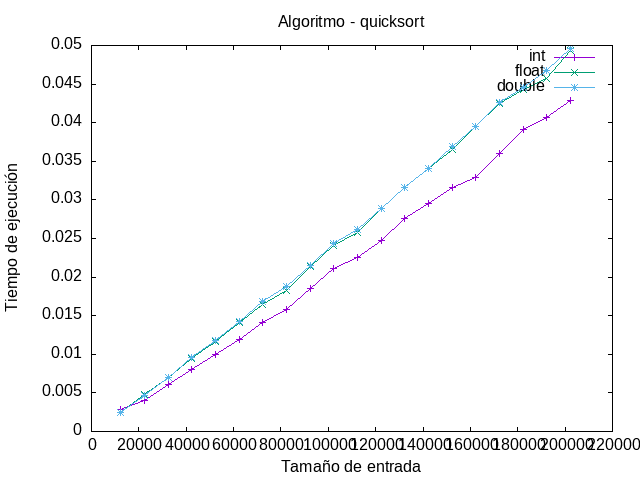
\includegraphics[width=\linewidth]{assets/Img/quicksort.png}
            \caption{Ejecución algoritmo quicksort}
            \label{fig:quicksort}
        \end{minipage}%
        \begin{minipage}{0.5\textwidth}
            \centering
            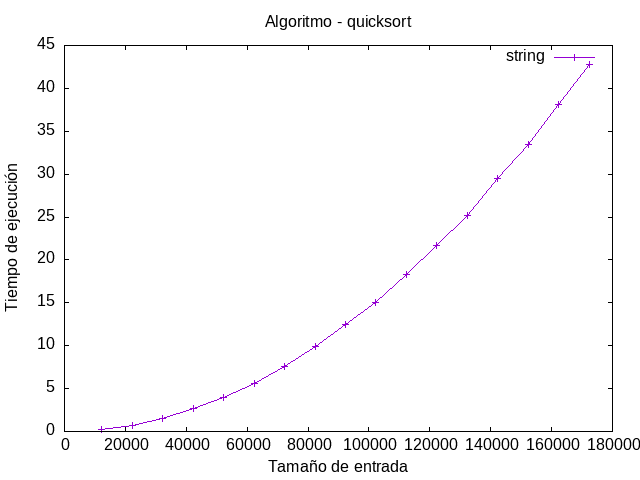
\includegraphics[width=\linewidth]{assets/Img/quicksortstring.png}
            \caption{Ejecución algoritmo quicksort con string}
            \label{fig:quicksortstring}
        \end{minipage}
    \end{figure}
    \begin{figure}[H]
        \begin{minipage}{0.5\textwidth}
            \centering
            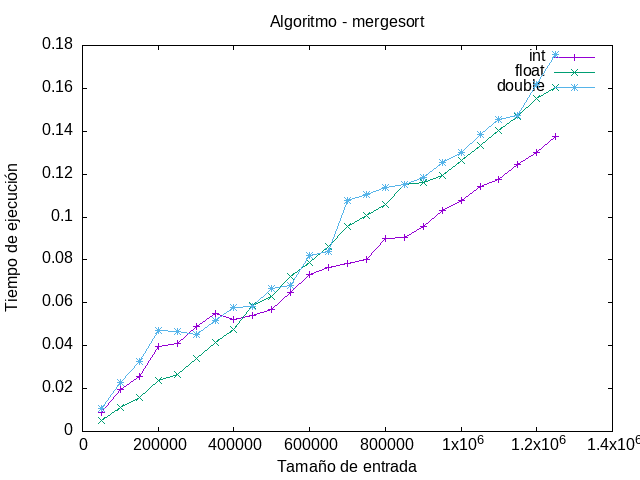
\includegraphics[width=\linewidth]{assets/Img/mergesort.png}
            \caption{Ejecución algoritmo mergesort}
            \label{fig:mergesort}
        \end{minipage}
        \begin{minipage}{0.5\textwidth}
            \centering
            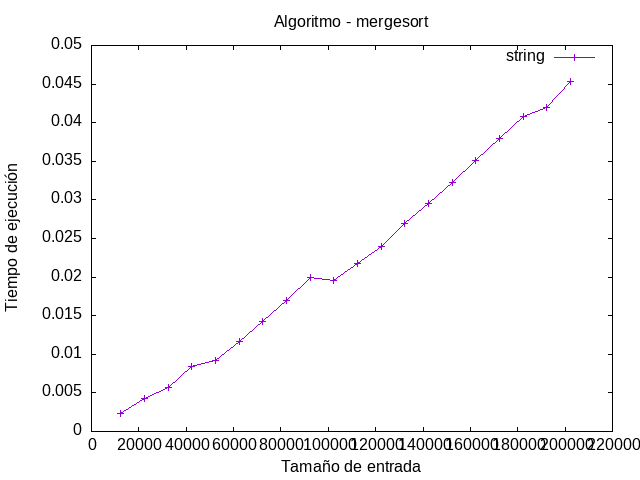
\includegraphics[width=\linewidth]{assets/Img/mergesortstring.png}
            \caption{Ejecución algoritmo mergesort con string}
            \label{fig:quicksortstring}
        \end{minipage}
    \end{figure}

    Pasamos ahora a estudiar los algoritmos con eficiencia \(O(n\log(n))\) los cuales veremos que son mas eficientes que los \(O(n^2)\)
    Si nos fijamos em la gráfica del quicksort veos que no hay casi diferencia entre los datos tipo float y double mientras que los datos tipo int son mas rapidos, 
    en el mergesort pasa justamente lo contrario , los tipos de datos double y float tardan menos en ser ordenados que los datos tipo int . 
    pero ambos son mas eficientes que los anteriormente vistos . 
    
    Si nos fijamos en las graficas de los algoritmos cuando los ejecutamos con datos de tipo string vemos que el mergesort gana en tiempo de ejecución al
    quicksort ya que en los casos donde hay datos repetidos el mergesort se comporta mejor que el quicksort debido a su implementacion.

    \subsection{Algoritmos Hanoi , Floyd y Fibbonaci}
    \begin{figure}[H]
        \begin{minipage}{0.5\textwidth}
            \centering
            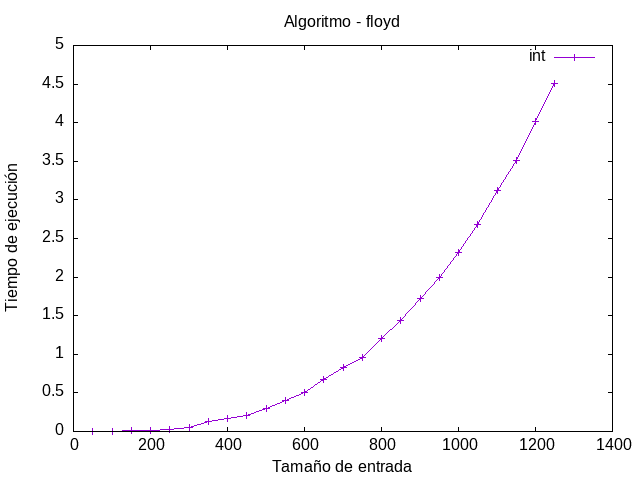
\includegraphics[width=\linewidth]{assets/Img/floydint.png}
            \caption{Ejecución algoritmo Floyd}
            \label{fig:floyd}
        \end{minipage}
        \begin{minipage}{0.5\textwidth}
            \centering
            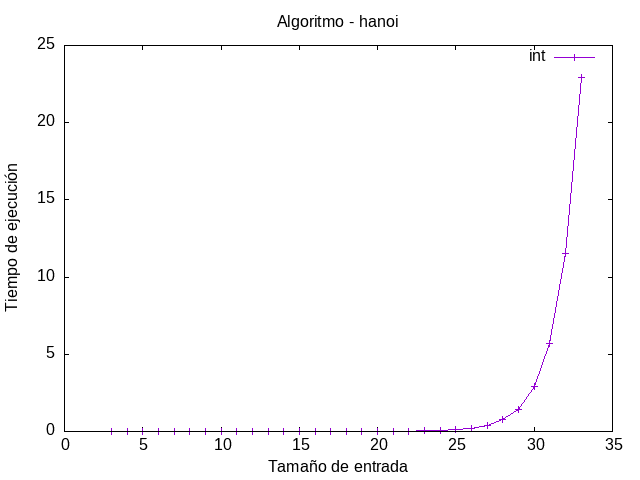
\includegraphics[width=\linewidth]{assets/Img/hanoiint.png}
            \caption{Ejecución algoritmo Hanoi}
            \label{fig:hanoi}
        \end{minipage}
    \end{figure}
    \begin{figure}[H]
        \begin{center}
            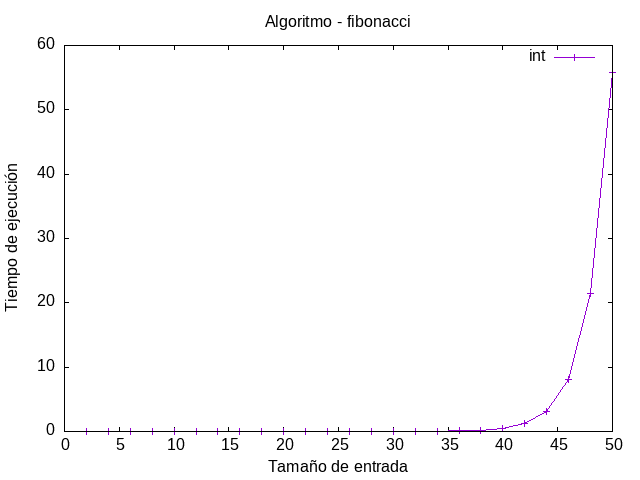
\includegraphics[width=0.5\linewidth]{assets/Img/fibonacciint.png}
            \caption{Ejecución algoritmo Fibonacci}
        \end{center}
    \end{figure}

    Por último pasamos a estudiar los algoritmos de Hanoi, Floyd y Fibonacci. Si nos fijamos en las gráficas de estos algoritmos vemos que el algoritmo de Floyd es el mas rapido ya que se trata de una algoritmo del orden \(O(n^3)\) por tanto 
    supera en velocidad a el algoritmo de Hanoi que es del orden \(O(2^n)\) y al algoritmo de Fibonacci que es del orden \(O((\frac{1+\sqrt{5}}{2})^n)\) siendo este ultimo el mas lento de todos.


    Como conclusion a este apartado hemos podido observar que los algoritmos de ordenación con eficiencia \(O(n^2)\) son mas lentos que los de eficiencia \(O(n\log(n))\) y que dependiendo del tipo de dato con el que se trabaje y de si hay datos repetidos o no habrá algoritmos a los que les afecte de manera 
    positiva como al mergesort o el de Inserción que pasa a ser practicamente logaritmico  y otros como el de burbuja o seleccion que se vean perjudicados por estos datos. 

\section{Conclusiones}
Como conclusión de la realización de esta memoria sobre el estudio de la eficiencia de difrentes algoritmos, podemos decir:
\begin{enumerate}
    \item En los algoritmos de ordenación pertenecientes a $O(n^2)$, su eficiencia teórica es muy fiel a los resultados obtenidos empíricamente.
    Es decir, son algorítmos que nos proporcionan una gran fiabilidad a la hora de tener que suponer un tiempo acorde a su fórmula teórica. Dentro
    de los cuales, el que mejor se comporta es el algortimo de inserción y el que lo hace peor el algorítmo de burbuja. De este último, podemos decir 
    que a la hora de ordenar vecotores con muchos datos repetidos, sea el caso del tipo string donde hay palabras que son más usadas, el algoritmo de 
    inserción toma especial relevancia debido a que su gráfica parece por momentos del tipo $f(x)=x$.En cuanto a los algoritmos de eficiencia $O(nlogn)$ 
    vemos que son más eficientes que los mencionados anteriormente. Sin embargo, no presentan una gráfica tan regular como los de eficiencia $O(n^{2})$.
    Por lo cual podrían ser menos fiables a la hora de ofrece un resultado más preciso. Por la parte de los algoritmos de Hanoi, Floyd y Fibonacci, al tener
    una eficiencia exponencial, puede ocurrir que haya grandes diferencias al introducir un nuevo elemento y aumentar en una unidad el tamaño del vector.
    \item Por lo que respecta a la parte del estudio híbrido, hemos observado que es una buena forma corroborar los resultados obtenidos en el estudio teórico.
    De aquí, podemos decir que el estudio teórico de los algoritmos, es una parte de gran relevancia a la hora del desarrollo de un proyecto ya que sus resultados
    son realmente cercanos a la realidad.
    \item Finalmente, como se puede observar en el apartado en el que comparamos un mismo método en diferentes ordenadores, vemos que el hardware donde se ejecute 
    el algoritmo tiene relevancia. Sin embargo, podemos afirmar que el estudio de la eficiencia de los algoritmos nos puede llevar más lejos a la hora de 
    reducir el tiempo de ejecución, siendo lo idóneo combinar esto junto a un buen hardware. 
    
\end{enumerate}

\end{document}